% !TEX root = ../document.tex

\chapter{现阶段发展及应用情况}

\section{DLR 的 AOS 实验项目}

\subsection{项目概述}

根据\ref{sec:space_based_ads-b_experiment_back}节的内容,我们得知 DLR 的 AOS 项目是世界上第一个天基 ADS-B 可行性验证实验项目。AOS 开发了一个 ADS-B 载荷,作为一个在轨演示器,搭载在 ESA 的 PROBA-Vegetation 卫星上,于 2013 年 5 月 7 日被发射到近地轨道上。AOS 是 DLR 空间系统研究所和 DLR 飞行指导研究所的合作项目,与卢森堡合作伙伴 SES TechCom Services 合作。

\renewcommand\arraystretch{1.5}
\begin{table}[!htb]
\centering
\caption{DLR 的 AOS 项目基本描述}
\label{tab:}
\begin{tabular}[b]{|p{2.2cm}<{\raggedleft}|p{13cm}<{\raggedright}|}
\hline
\textbf{目标} & 证明星基 ADS-B 监视的可行性 \par
            搭载于 ESA 的 Proba-V 卫星上的在轨演示器将验证一些关键参数,例如目标截获率、检测率和验证概率 \\
\hline
\textbf{项目持续时间} & 2011 年第一季度至 2014 年第二季度末 \\
\hline
\textbf{合作方} & Institute of Space Systems (RY) in Bremen, Germany \par\par
        Institute for Flight Guidance (FL) in Braunschweig, Germany \\
\hline
\textbf{贡献} & Institute RY: 开发和组装符合空间要求的 ADS-B 接收机和天线\par
Flight Calibration Services: 开发 ADS-B 接收机\par
Institute FL: ADS-B 数据的验证与评估 \\
\hline
\textbf{更多的合作} & RY with SES-ASTRA / ESA: 提供数据服务器 \\
\hline
\end{tabular}
\end{table}

\renewcommand\arraystretch{1.5}
\begin{table}[!htb]
\centering
\caption{ESA 的 Proba-V 小卫星任务描述}
\label{tab:esa_Proba-V_mission}
\begin{tabular}[b]{|p{2.5cm}<{\raggedleft}|p{12cm}<{\raggedright}|}
\hline
\textbf{主承包商} & QinetiQ Space nv \\
\hline
\textbf{卫星质量} & 约 140 kg\\
\hline
\textbf{运载火箭 }& Vega 火箭\\
\hline
\textbf{发射日期} & 2013 年 5 月 7 日 \\
\hline
\textbf{发射场} & 法属圭亚那航天中心(库鲁)\\
\hline
\textbf{发射提供商} & Arianespace \\
\hline
\textbf{轨道} & 太阳同步轨道,海拔 820 公里,倾角 98.73$^\circ$,飘移限制在 10:30 AM 到 11:30 AM  \\
\hline
\textbf{通信} & 卫星的控制与通信通过比利时 Redu 地面站 \\
\hline
\textbf{主要任务} & 植被扫描仪 \\
\hline
\textbf{载荷} & ADS-B、高能粒子传感器、氮化镓 X 波段功率放大器 \\
\hline
\end{tabular}
\end{table}

ESA Proba-V 卫星自 2013 年 5 月 7 日起进入地球轨道, 其有效载荷包括一个专用接收器,用于接收飞机 ADS-B 信号。5 月 23 日,该实验首次开启,在两小时内在 820 公里的高度记录了 12000 条 ADS-B 信息。飞越苏格兰的 A320 飞机是 DLR 新型接收机从太空“看到”的第一架飞机,证明可以从太空跟踪飞机。


\subsection{体系结构}

Proba-V 上的 ADS-B 接收器由卢森堡的 DLR 和 SES TechCom 提供,主要目的是在飞行代表性配置中测试(空间限定)ADS-B 电路板以评估 \acs{TID}。

ADS-B 接收器(1090ES RX)的基本设计概念是单转换超外差接收机,由 1090MHz 下变频调至中频 70MHz,70MHz 下的 \acs{IF} 采样由一个 105Msps(每秒兆采样次数)的 16 位 \acs{ADC} 完成。该 ADS-B 单转换超外差接收机概念如图\ref{fig:dlr_ads-b_receiver}所示\upcite{e2}。

\begin{figure}[!htb]
\centering
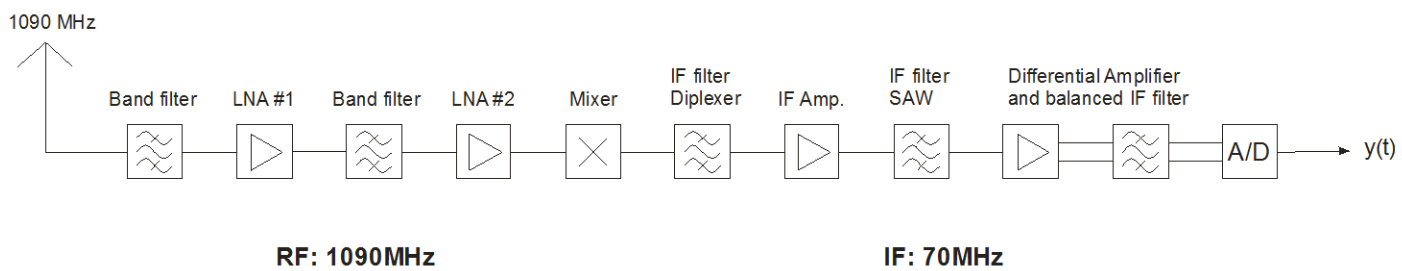
\includegraphics[width=15cm]{pic/dlr_ads-b_receiver.png}
\caption{单转换超外差接收机\protect\footnotemark}
\label{fig:dlr_ads-b_receiver}
\end{figure}

\footnotetext{图片来源:参考文献\cite{e2}}

\begin{figure}[!htb]
\centering
\subfigure[载荷原型]{
\begin{minipage}[b]{0.3\linewidth}
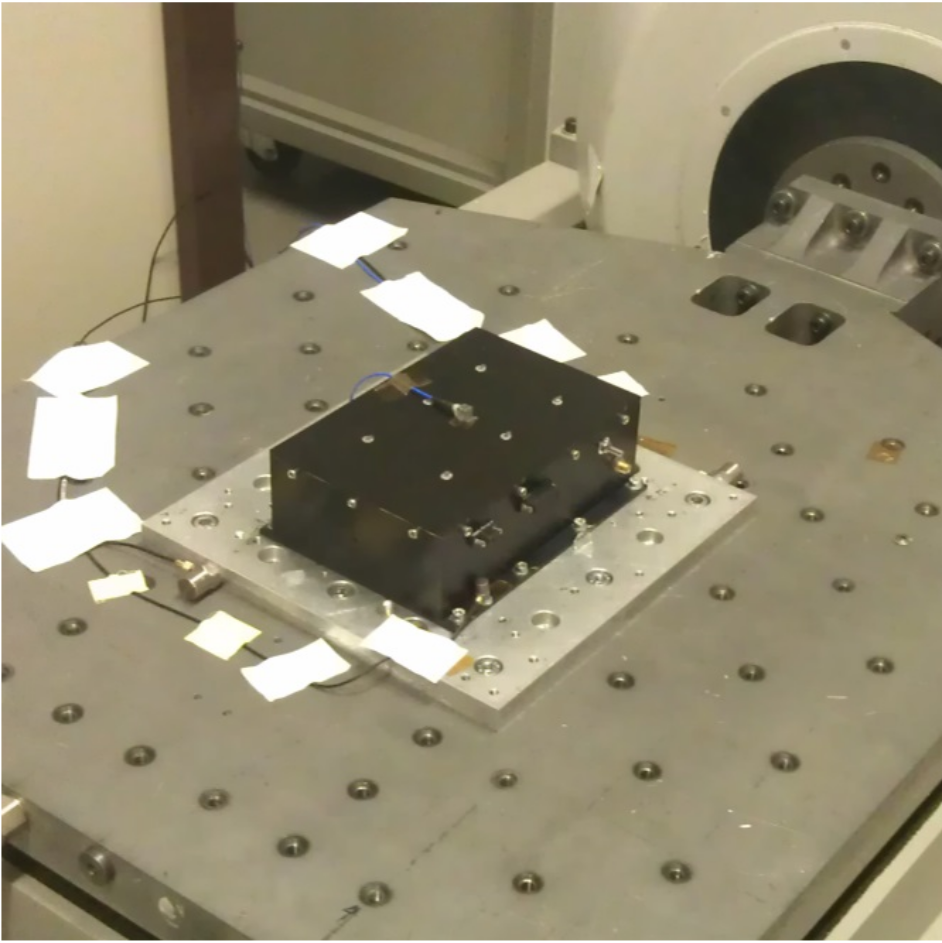
\includegraphics[width=1\linewidth]{pic/aos_ads-b_payload_2.png}
\end{minipage}}
\subfigure[安装位置]{
\begin{minipage}[b]{0.3\linewidth}
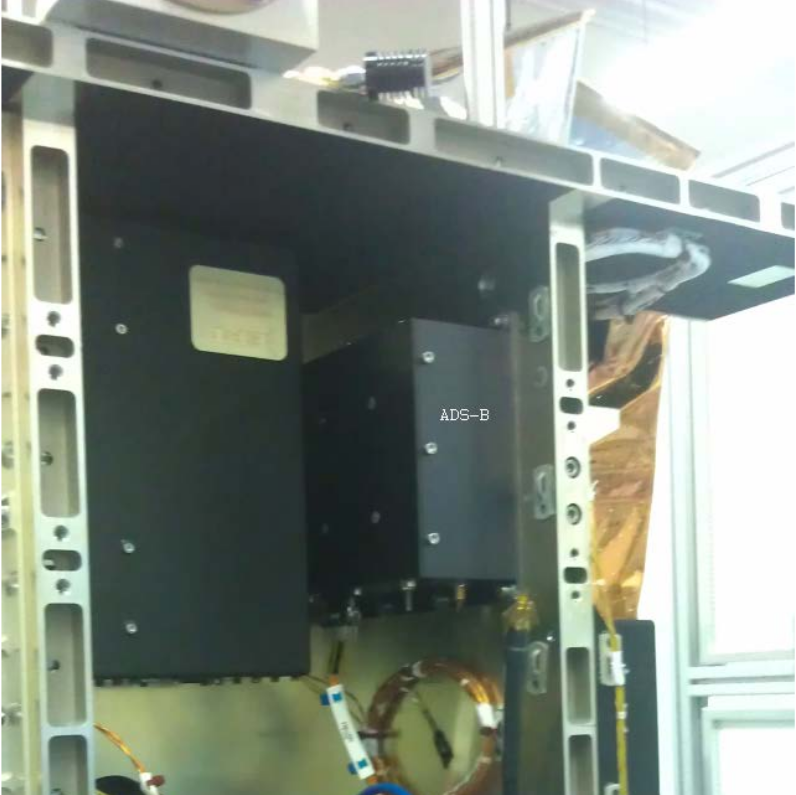
\includegraphics[width=1\linewidth]{pic/aos_ads-b_payload_1.png}
\end{minipage}}
\subfigure[卫星原型]{
\begin{minipage}[b]{0.3\linewidth}
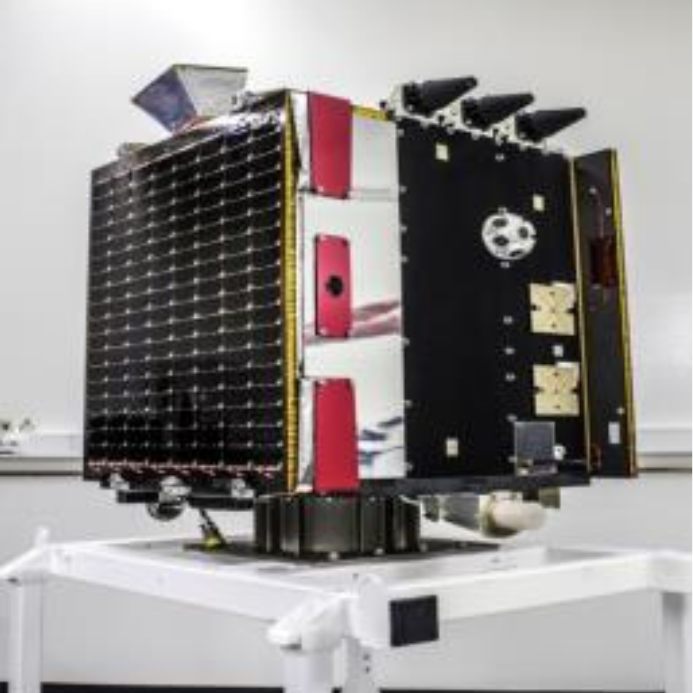
\includegraphics[width=1\linewidth]{pic/aos_ads-b_payload_3.png}
\end{minipage}}
\caption{Proba-V 卫星上搭载的 ADS-B 载荷\protect\footnotemark}
\label{fig:aos_ads-b_payload}
\end{figure}

\footnotetext{图片来源:参考文献\cite{e2ppt}}

\begin{figure}[!htb]
\centering
\begin{minipage}[t]{0.48\textwidth}
\centering
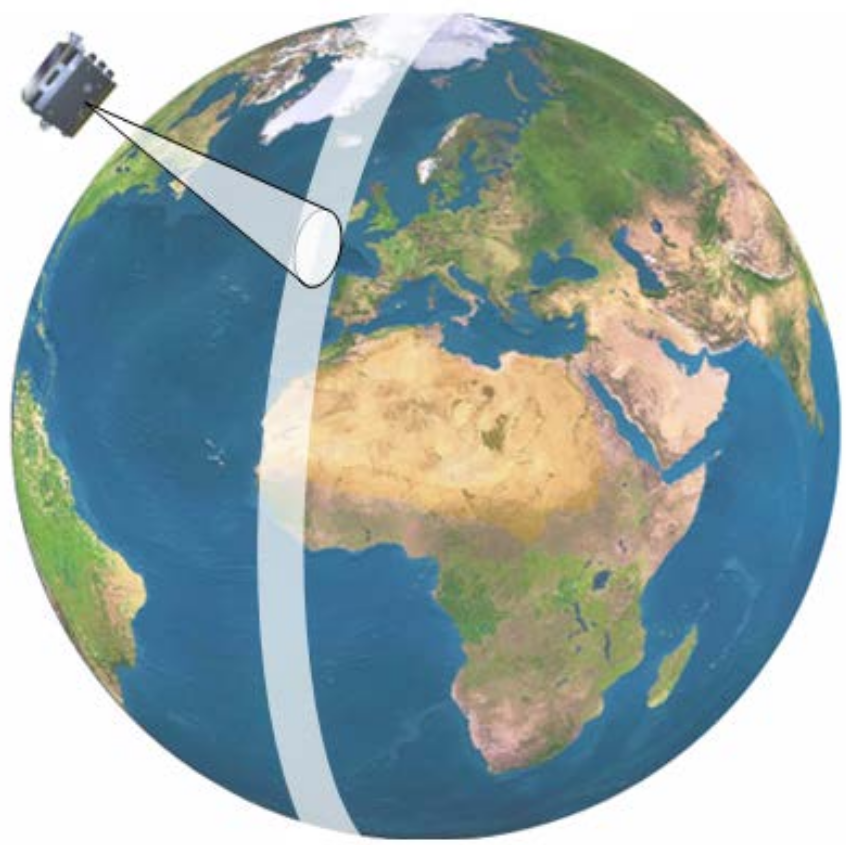
\includegraphics[width=6cm]{pic/aos_in_orbit.png}
\caption{技术验证阶段的单颗卫星\protect\footnotemark}
\label{fig:aos_in_orbit}\footnotetext{图片来源:参考文献\cite{e2ppt}}
\end{minipage}
\begin{minipage}[t]{0.48\textwidth}
\centering
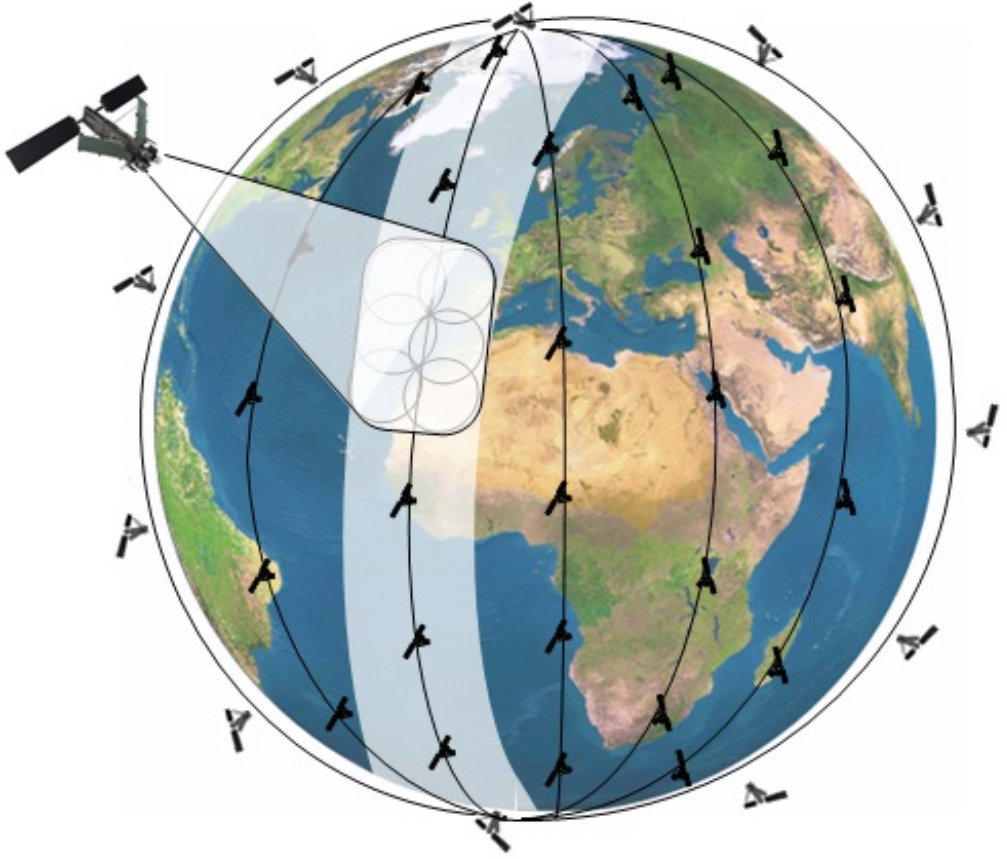
\includegraphics[width=7.2cm]{pic/aos_in_future.png}
\caption{未来全球卫星组网方案}
\label{fig:aos_in_future}\footnotetext{图片来源:参考文献\cite{e2ppt}}
\end{minipage}
\end{figure}


\subsection{实验结果}

图\ref{fig:ADS-B_Auto6}展示了 2014 年 2 月 11 日在世界范围内记录的飞机航迹,每个红点代表卫星在其轨道上通过飞机时所看到的飞机航迹段。Proba-V 卫星的天线覆盖范围为纵向约 1200 公里,横向延伸至卫星飞行方向 500 公里,可逐条扫描全球空域。

\begin{figure}[!htb]
\centering
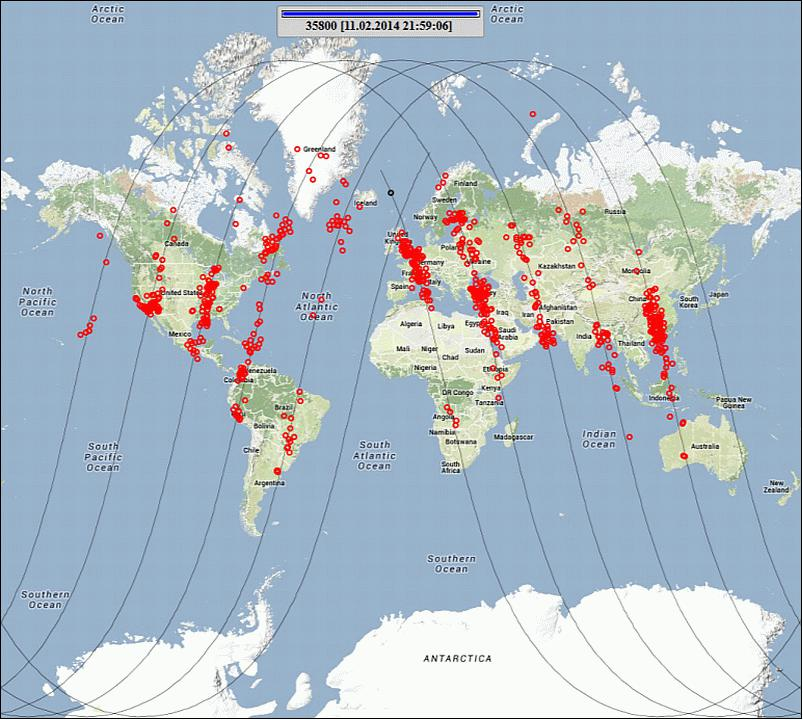
\includegraphics[width=10cm]{pic/ADS-B_Auto6.jpeg}
\caption{AOS 在世界范围内记录的飞机航迹(2014 年 2 月 11 日)\protect\footnotemark}
\label{fig:ADS-B_Auto6}
\end{figure}

\footnotetext{图片来源:参考文献\cite{e2ppt}}

在空间接收 ADS-B 报文的最重要方面是卫星上 1090 MHz 扩展电文信号的接收条件。与基于地面的 ADS-B 监视相比,陆基 ADS-B 最大接收范围可达 300 公里,而在 820 公里高度轨道运行的 LEO 卫星与飞机之间的信号路径要长得多,这导致 ADS-B 的信号电平较低。接收器必须通过相关处理几乎在噪声水平上检测 S 模式信号。

实验得到了卫星天线覆盖区中不同区域接收到的 ADS-B 报文数量分布的足迹,如图\ref{fig:ADS-B_Auto5}所示,该图显示了 2014 年 5 月收到的所有位置消息的足迹。值得注意的是两个峰值,一个在卫星运动方向前方,峰值较低,另一个在卫星运动方向后方,峰值较高。这个谱的分布是不对称的,这由许多原因引起,比如卫星上的贴片天线的安装位置不对称、安装在卫星下侧的其他设备和在下表面的前边缘上突出的太阳能电池板。

\begin{figure}[!htb]
\centering
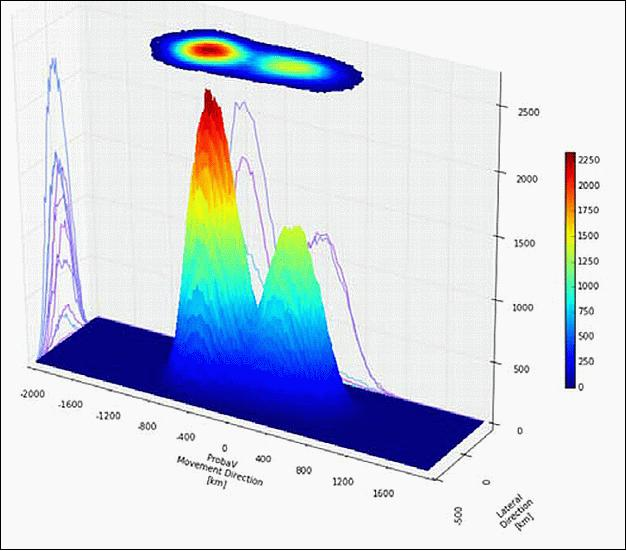
\includegraphics[width=10cm]{pic/ADS-B_Auto5.jpeg}
\caption{所有接收到的位置信息在天线覆盖区中的分布足迹\protect\footnotemark}
\label{fig:ADS-B_Auto5}
\end{figure}

\footnotetext{图片来源:参考文献\cite{e2ppt}}

直方图的峰值可以通过卫星的接收天线和飞机的发射天线的天线辐射图来解释。图\ref{fig:ADS-B_Auto4}显示了安装在 Proba-V 卫星最低点面板上的 ADS-B 贴片天线的实测辐射图。合成的天线辐射图在卫星移动方向整体呈椭圆形状,最大灵敏度略低于卫星下方的最低点方向。

飞机装有两个 ATC 天线,一个在机身顶部,一个在机身底部,它们交替发射。由于几何因素限制,卫星将接收来自顶部天线的信号。顶部天线典型的垂直天线辐射模式如图\ref{fig:antenna_of_plane}所示。

\begin{figure}[!htb]
\centering
\begin{minipage}[t]{0.48\textwidth}
\centering
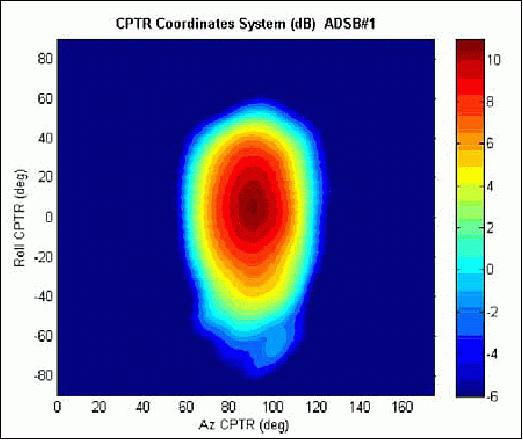
\includegraphics[width=7.5cm]{pic/ADS-B_Auto4.jpeg}
\caption{Proba-V 卫星天线辐射图\protect\footnotemark}
\label{fig:ADS-B_Auto4}\footnotetext{图片来源:参考文献\cite{e2ppt}}
\end{minipage}
\begin{minipage}[t]{0.48\textwidth}
\centering
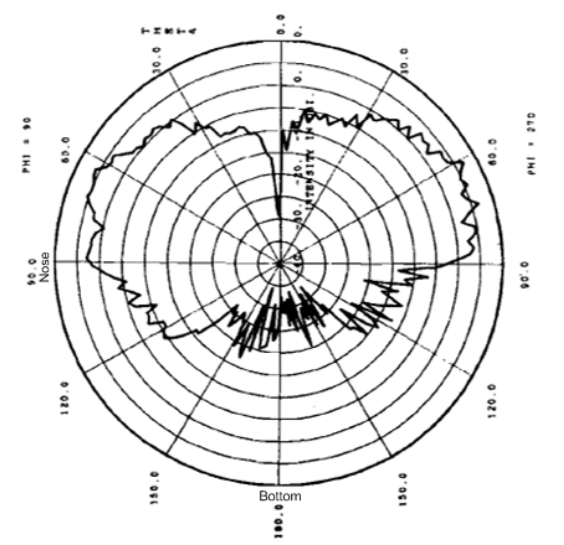
\includegraphics[width=6.5cm]{pic/antenna_of_plane.png}
\caption{顶部安装的 L 波段天线的垂直天线辐射图\protect\footnotemark}
\label{fig:antenna_of_plane}\footnotetext{图片来源:参考文献\cite{e2ppt}}
\end{minipage}
\end{figure}

\subsection{项目意义}

这次星载 ADS-B 接收验证实验的创举,将带来更多的在轨验证任务。ESA 与 Thales 德国签订合同,开发下一代 ADS-B 系统,该系统正在按计划进行,同时带来了卢森堡航天界(如 LuxSpace)的大力参与,将 TRITON 微小卫星平台作为以后的实验平台\upcite{h2}。

Proba-V 卫星实验项目取得了多个成果,主要包括:

\begin{itemize}
    \item 接收器的 \acs{FPGA} 固件中包含一项特殊功能:允许上载新配置文件并通过远程访问激活这些配置。到目前为止,在任务运行期间,已成功测试了几次;

    \item 开发了改进的 S 模式相关机制,这得益于脉冲序列从第一个到第五个前导脉冲的相位相干性。在实验室测试中,可以显示报文检测率显著增加;

    \item 通过为 DF17 中的 112 个 S 模式数据位生成并保存“低置信度位”,增加了一次可以提高后处理报文解调成功率的机会;

    \item 卫星上的 ADS-B 接收器是同类中的第一个实验,接收从飞机发射的 1090ES ADS-B 电文信号。因此无法根据以往经验或任何结果进行系统设计。
\end{itemize}

Proba-V 卫星在实验中也遇到了一些困难,主要包括:

\begin{itemize}
    \item 由于卫星在大约 820 公里的高度,而飞机在 0 到 12 公里的高度,距离会导致接收的信号幅度过低从而导致信号丢失;

    \item 由于卫星天线垂直辐射图和飞机天线垂直辐射图的形状不同,会导致信号损失;

    \item 当到达卫星 ADS-B 天线的消息在时间上重叠(交织)时,ADS-B 接收机无法对其进行解码;

    \item 卫星的速度约为 27000 公里/小时,这导致每个检测到的飞机的观察时间有限,最多约 3 分钟。
\end{itemize}

这些困难提供了巨大的借鉴意义,为星基 ADS-B 技术发展中探明了一些需要克服的难点问题。

\section{丹麦 GOMX 实验项目}

\subsection{项目概述}

GOMX 平台是商业上可获得的立方体卫星套件,由丹麦奥尔堡的 GomSpace ApS 提供。GomSpace 是一家创业型公司,于 2007 年成立为私人有限公司。该平台非常适合以技术研究,低成本科学和商业概念验证任务为重点的具有成本效益的任务。GOMX(GomSpace Express)平台是开发空间技术能力的客户工具\upcite{h14}。

\subsubsection{GOMX-1 -> GATOSS}

GATOSS 是 GomSpace 的纳米卫星平台,基于两个单元 GomSpace Express(GOMX)平台的立方体卫星,在对应于平台上部 14 厘米的体积内提供 1.2 千克的有效载荷\upcite{h14}。GATOSS 卫星项目的相关参数如图\ref{fig:GATOSS_AutoD}所示。

GOMSpace 的 GOMX-1 在发布后改名为 GATOSS(Global Air Traffic Awareness and Optimizing through Spaceborne Surveillance,全球空中交通态势和通过星载监视进行优化),是一款学生建造的业余无线电 2U 立方体卫星。该任务是在政府研究基金的赞助下进行的,涉及与空间有关的无线电研究。该卫星的目标是确定若干子系统的性能并提供广泛的飞行数据。

GOMX-1 具有有效载荷,能够通过接收飞机发出的 ADS-B 信号,从太空进行跟踪跨洋飞行。ADS-B 信号目前在地面接收机覆盖的区域内用于空中交通管制,但由于其范围有限,目前尚未在海洋上使用。具有敏感软件无线电(SDR)有效载荷的 GOMX-1 卫星将首次证明 ADS-B 信号可以从太空接收,并用于为空中交通管制中的关键利益相关者提供更高的全球态势感知能力。

该任务还将测试使用开源立方体卫星空间协议进行包括空间链接在内的完整任务。

作为学期项目的一部分,奥尔堡大学的 15 名学生积极参与了这种有效载荷的开发。\upcite{h13}

\begin{figure}[!htb]
\centering
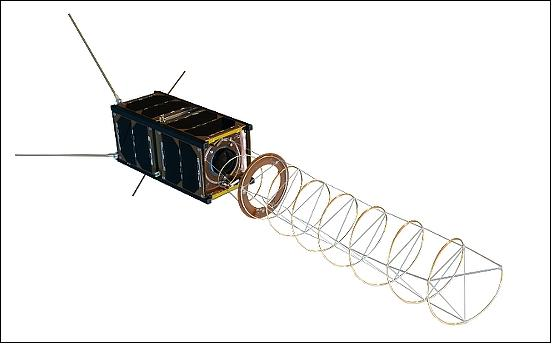
\includegraphics[width=11cm]{pic/GATOSS_AutoD.jpeg}
\caption{GOMX-1(GATOSS)卫星\protect\footnotemark}
\label{fig:GATOSS_AutoD}
\end{figure}

\footnotetext{图片来源:参考文献\cite{h13}}

\renewcommand\arraystretch{1.5}
\begin{table}[!htb]
\centering
\caption{GATOSS 卫星项目相关参数\protect\footnotemark}
\label{tab:gatoss_satellite_program}
\begin{tabular}[b]{|p{3cm}<{\raggedleft}|p{6cm}<{\raggedright}|}
\hline
国家 & 丹麦  \\
\hline
类型/应用 &  技术,交通监控  \\
\hline
运营商 &  GOMSpace  \\
\hline
承办单位 &  GOMSpace  \\
\hline
设备 & ADS-B 接收器  \\
\hline
组态 & 2 单元立方体卫星  \\
\hline
推进 & 无 \\
\hline
能源 & 太阳能帆板,电池  \\
\hline
寿命 &  \\
\hline
质量 & 2 kg  \\
\hline
轨道 & 593 km × 818 km,97.78$^\circ$  \\
\hline
发射日期 & 2013 年 11 月 21 日 \\
\hline
运载火箭 & Dnepr \\
\hline
\end{tabular}
\end{table}

\footnotetext{数据来源:参考文献\url{h13}}

\subsubsection{GOMX-3}

GOMSpace 的 GOMX-3 是 3 单元立方体卫星,用于评估太空中的几个组件。GOMX-3 卫星项目相关参数如图\ref{fig:gomx-3__1}所示。

GOMX-3 将使用 L 波段可重新配置的软件定义无线电有效载荷来演示飞机 ADS-B 信号接收和对地静止通信卫星点波束信号质量。由 Syrlinks 开发并由法国航天局 CNES 资助的小型高数据速率 X 波段发射机也将作为第三方有效载荷飞行。

卫星由 HTV 5 货船运送到国际空间站。它于 2015 年 10 月 5 日从国际空间站部署。它于 2016 年 10 月 18 日重新进入大气层销毁。\upcite{h16}

\begin{figure}[!htb]
\centering
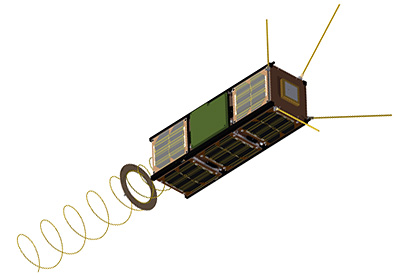
\includegraphics[width=9cm]{pic/gomx-3__1.jpg}
\caption{GOMX-3 卫星\protect\footnotemark}
\label{fig:gomx-3__1}
\end{figure}

\footnotetext{图片来源:参考文献\cite{h16}}

\renewcommand\arraystretch{1.5}
\begin{table}[!htb]
\centering
\caption{GOMX-3 卫星项目相关参数\protect\footnotemark}
\label{tab:gatoss_satellite_program}
\begin{tabular}[b]{|p{3cm}<{\raggedleft}|p{6cm}<{\raggedright}|}
\hline
国家 & 丹麦 \\
\hline
类型/应用 &  技术,交通监控 \\
\hline
运营商 &  GOMSpace \\
\hline
承办单位 &  GOMSpace \\
\hline
设备 &  \\
\hline
组态 & 3 单元立方体卫星 \\
\hline
推进 & 没有 \\
\hline
能源 & 太阳能帆板,电池 \\
\hline
寿命 & 1 年 \\
\hline
质量 & 4 kg \\
\hline
轨道 & 395 km × 408 km,51.64$^\circ$ \\
\hline
发射日期 & 2015 年 8 月 19 日 \\
\hline
运载火箭 & H-2B-304 \\
\hline
\end{tabular}
\end{table}

\footnotetext{数据来源:参考文献\url{h16}}

\subsection{体系结构}

\subsubsection{GOMX-1 -> GATOSS}

星载 ADS-B 的目的是将敏感接收机放置在 LEO 的卫星上,该轨道可接收 ADS-B 信号并将其传递给相关的利益攸关方。GomSpace 的星载 ADS-B 概念如图\ref{fig:GATOSS_Auto5}所示,GomSpace 正在研究利用纳米卫星提供星载 ADS-B 服务的两个概念。

离线数据:一小队卫星(3-6 颗)对空域进行采样,主要为离线统计处理提供信息。经过一个或多个地面站时,有延迟的数据被传递至下行链路。

在线数据:一个较大的卫星网络(40-70 颗)通过地球同步数据中继卫星近乎实时地连接到空中交通管制基础设施。这可以使用例如用于 Inmarsat BGAN 网络的 SB-SAT 来实现,该网络正在开发中。\upcite{h14}

\begin{figure}[!htb]
\centering
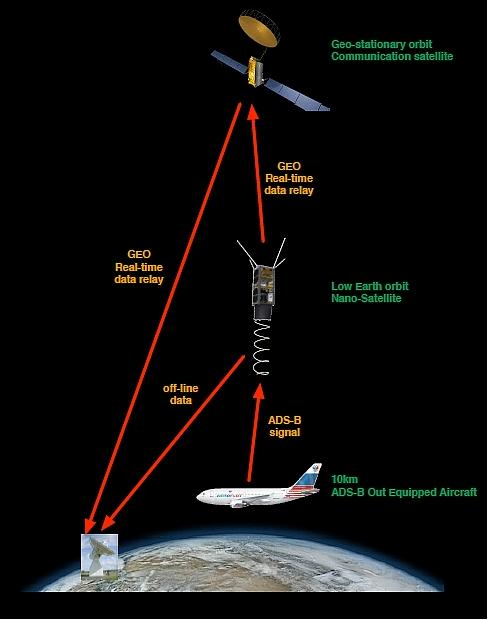
\includegraphics[width=9cm]{pic/GATOSS_Auto5.jpeg}
\caption{GomSpace 的星载 ADS-B 概念图\protect\footnotemark}
\label{fig:GATOSS_Auto5}
\end{figure}

\footnotetext{图片来源:参考文献\cite{h14}}

虽然确实是一个有趣的想法,但是星载 ADS-B 需要带来经济效益才能生存并值得投资。对于仅是适度投资的离线数据概念,可以通过分析提供由卫星采样的飞行验证信息的过去数据来生成值。此信息可用于以下示例:

\begin{itemize}
    \item 航路收费计算的改进使收益率比已公布的飞行计划计算的收费增加 1-2\%

    \item 飞机航线和先前地点的第二个来源,作为国家安全情报收集的输入

    \item 根据星载 ADS-B 记录的使用模式改进海洋空域作业程序,以提高空域效率
\end{itemize}

显然,随着星座中卫星数量的增加,可以提供更好的服务。对于在线数据概念,需要大量投资,提供全球空中交通状况的全时态势感知。GomSpace 估计,全球覆盖的全面部署的星载 ADS-B 基础设施对空中交通部门的潜在价值大约为十亿美元,其中很大一部分可能在北大西洋地区产生。\upcite{h14}

图\ref{fig:GATOSS_Auto4}中提供了 ADS-B 接收器有效负载的框图。该天线是图\ref{fig:GATOSS_AutoD}所示的可展开螺旋天线,在 1090 MHz 时提供 10dB 的增益。

\begin{figure}[!htb]
\centering
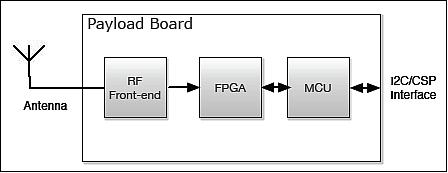
\includegraphics[width=11cm]{pic/GATOSS_Auto4.jpeg}
\caption{GATOSS 上的 ADS-B 接收器框图\protect\footnotemark}
\label{fig:GATOSS_Auto4}
\end{figure}

\footnotetext{图片来源:参考文献\cite{h14}}

RF 前端提供信号的放大和初始下变频。为了补偿由于接收器在空间中的位置而导致的路径损耗增加,与系统的 80 NM 标称范围形成对比,RF 前端经过精心设计,可提供所需的灵敏度,以便能够对信号进行解码。

FPGA 对下变频信号进行采样并运行解码算法。在任务期间可以使用新的位代码重新配置 FPGA,并且该功能将用于在任务期间基于在空间中操作所获得的反馈来改善有效载荷的操作性能。

FPGA 将解码后的包传输到微控制器单元,该单元将数据存储在(内存中)数据库中,该数据库可通过 CSP(立方体卫星空间协议)网络查询,从而提供广泛的机会来提取 ADS-B 数据和系统性能的元数据。\upcite{h14}

\subsection{实验成果}

\subsubsection{GOMX-1 -> GATOSS}

2013 年 11 月 25 日:GATOSS 现已全面投入使用。姿态控制系统使航天器从相当高的倾斜速率中脱离,并且部署了包括螺旋天线的所有可展开部件。两个有效载荷都处于完全运行状态。主要有效载荷-软件无线电 ADS-B 接收器,已经接收到大量的航空器信号,表明螺旋天线上的链路预算好于预期。

2014 年 2 月 19 日:GATOSS 航天器名义上运行。该项目目前正在使用卫星捕获原始和解码 ADS-B 数据的各种样本,以便进行分析,并将其输入下一代接收机。

截至 2013 年 12 月 GATOSS 收到的几架飞机位置的图像如图\ref{fig:GATOSS_Auto6}所示。

\begin{figure}[!htb]
\centering
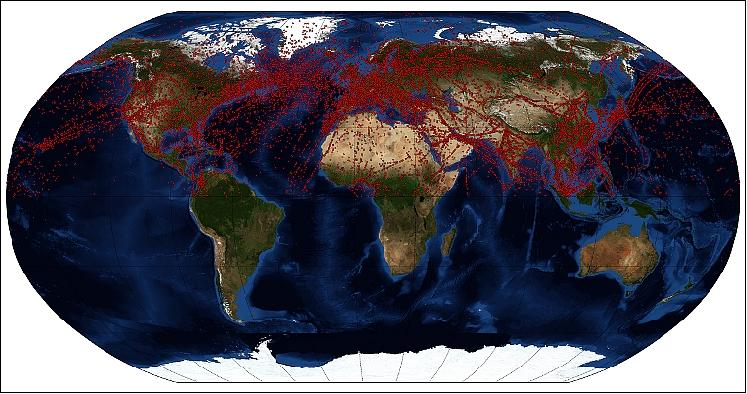
\includegraphics[width=13cm]{pic/GATOSS_Auto6.jpeg}
\caption{截至 2013 年 12 月 GATOSS 收到的几架飞机位置的初步图\protect\footnotemark}
\label{fig:GATOSS_Auto6}
\end{figure}

\footnotetext{图片来源:参考文献\cite{h14}}

马来西亚航空 370 航班(MH370 是定期从吉隆坡飞往北京的国际客运航班,于 2014 年 3 月 8 日失去与空中交通管制的联系。马来西亚航空 MH370 失踪时期,GOMX-1 卫星正在空间中运行,虽然 GOMX-1 多次从 MH370 飞机的特定波音 777 机身上接收到 ADS-B 数据,然而,遗憾的是,当 MH370 消失时,GOMX-1 卫星并未在该区域上空。如果 GOMX-1 进入该地区,至少可能有空间 ADS-B 数据有助于准确了解飞机应答器何时关闭以及该时飞机的位置\upcite{h17}。

\subsubsection{GOMX-3}

GomX-3 在 2016 年 4 月的前六个月内从国际空间站发布以来接收到的飞行中的飞机信号已经有数百万个,如图\ref{fig:ef59906e566da47d7760e54dd9c6662d}所示,这些信号可以提供飞行信息,如速度,位置和高度。

与 FlightRadar24 和 Airbus Defense and Space 一起,对北大西洋上空的飞机进行了实时跟踪,直接融入 FlightRadar24 基础设施。目前该卫星已经进入大气层被销毁。

\begin{figure}[!htb]
\centering
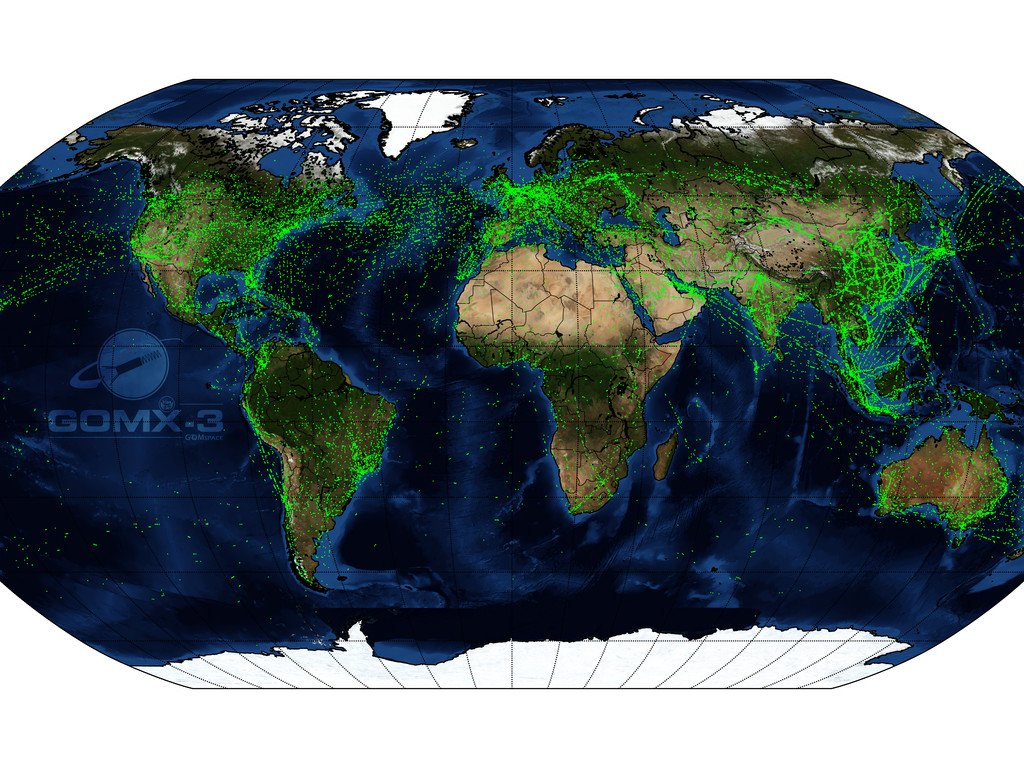
\includegraphics[width=11cm]{pic/ef59906e566da47d7760e54dd9c6662d.jpg}
\caption{GomX-3 在 2016 年 4 月的前六个月内从国际空间站发布以来接收到的飞行中的飞机信号\protect\footnotemark}
\label{fig:ef59906e566da47d7760e54dd9c6662d}
\end{figure}

\footnotetext{图片来源:参考文献\cite{h16}}



\section{Aireon 星基 ADS-B 系统}

\subsection{系统概述}

Aireon 星基 ADS-B 系统是搭载于第二代铱星(Iridium Next)卫星上的,作为第二代铱星星座系统提供服务的一部分。

\subsubsection{利益攸关方}

Aireon 的星基 ADS-B 系统的利益攸关方如表\ref{tab:stakeholders_of_Aireon_ads-b}所示。

\renewcommand\arraystretch{1.5}
\begin{table}[!htb]
\centering
\caption{Aireon 星基 ADS-B 系统的利益攸关方}
\label{tab:stakeholders_of_Aireon_ads-b}
\begin{tabular}[b]{|p{6cm}<{\raggedleft}|p{8cm}<{\raggedright}|}
\hline
\textbf{Iridium} & 卫星星座的拥有者和运营方 \\
\hline
\textbf{Aireon} & Iridium 和 NAV CANADA 的合资企业,旨在建立 ADS-B 服务 \\
\hline
\textbf{TAS(Thales Alenia Space)}& 卫星建造商,与 Iridium 签订合同 \\
\hline
\textbf{Harris Corporation} & ADS-B 有效载荷的建造商,与 Aireon 签订合同 \\
\hline
\textbf{ITT-Exeils} & 系统工程支持提供商,与 Aireon 签订合同,是处理和分销子系统的建造商 \\
\hline
\textbf{NAV CANADA} & Aireon 的投资方,为 ADS-B 服务启动客户 \\
\hline
\end{tabular}
\end{table}

\subsubsection{背景}

2012 年 11 月,铱星通信公司与 NAV CANADA 合资建立了 Aireon LLC 公司,这家合资企业将允许全球各地的空中交通管理机构持续跟踪世界各地的飞机。有史以来第一次,全球各地的 ANSP 将能够从极地到极地的追踪飞机,包括海洋空域和偏远地区。这将为航空业带来显著效益,包括大幅节省燃料,减少温室气体排放,提高安全性和效率等。该合资企业将在 FAA、行业和世界主要 ANSP 之间的 \acs{PPP} 下运营。

NAV CANADA 是一家加拿大的 ANSP,是 Aireon 的第一个客户,因为它管理着第二大空中导航服务并且是跨洋服务最大的提供商。

2014 年,Aireon LLC 成为 NAV CANADA、IAA(Irish Avation Authority)、ENAV(Ente Nazionale per l'Assistenza al Volo, Italy)、NAVIAR (Navigation Via Air, Denmark) 和 Iridium 共同的合资企业,用于融资、开发、部署并使用星基 ADS-B 接收器运行全球解决方案,以便在世界任何地方跟踪和监控飞机。\upcite{h2}

\subsubsection{铱星历史}

\begin{itemize}
    \item \textbf{初代铱星}

    铱星卫星星座(Iridium satellite constellation)是在 20 世纪 90 年代初构想出来的,主要目的是提供全球卫星通讯服务。早期的计算表明需要 77 颗卫星,因此取名为铱星,这是由于这个卫星星座系统的结构类似于化学元素依(原子序数为 77,原子核周围有 77 个电子)。后来的事实证明,只需要 66 颗卫星即可完成对地球的全面覆盖。

    第一代铱星星座由 Iridium SSC(铱星通讯公司的前身) 开发,由摩托罗拉赞助。这些卫星于 1997-2002 年部署。第一代铱星卫星由美国、俄罗斯和中国的运载火箭发射,其中美国的 Delta II 火箭发射其中的 60 颗卫星;俄罗斯的 Proton-K/DM2 火箭发射其中的 21 颗卫星,1 枚 Rokot/Briz-KM 火箭发射其中的 2 颗;中国的“长征 2 号丙改进型”火箭发射其中的 12 颗卫星。

    第一代铱星全球覆盖于 2002 年完成,虽然系统满足其技术要求,但在市场上并不成功。传统地面移动通信几乎完全占领市场,铱星电话无法形成稳定的客户群,摩托罗拉公司未能获得足够的收入来偿还与建造星座相关的债务,而铱星公司则于 2000 年 3 月 17 日宣布破产,这是当时美国历史上最大的破产案。

    在最初的铱星公司宣布破产后,铱星星座系统仍然存在。铱星在 2001 年接受不足建设投资的 1\% (4800 万美元)新注资后起死回生,美国军方是它主要客户,还被用于伊拉克战争,负责美军以及美军与盟军之间的协调行动。2010 年,铱星通信与波音公司就卫星网络的维护,运行和支持达成了长期协议,波音运营星座,并为铱星的卫星控制系统提供支持\upcite{h4}。

    尽管基于 LM-700A 型号的原始卫星预计设计寿命仅为 8 年,但 2002 - 2017 年没有发射新卫星来补充星座。

    \begin{figure}[!htb]
    \centering
    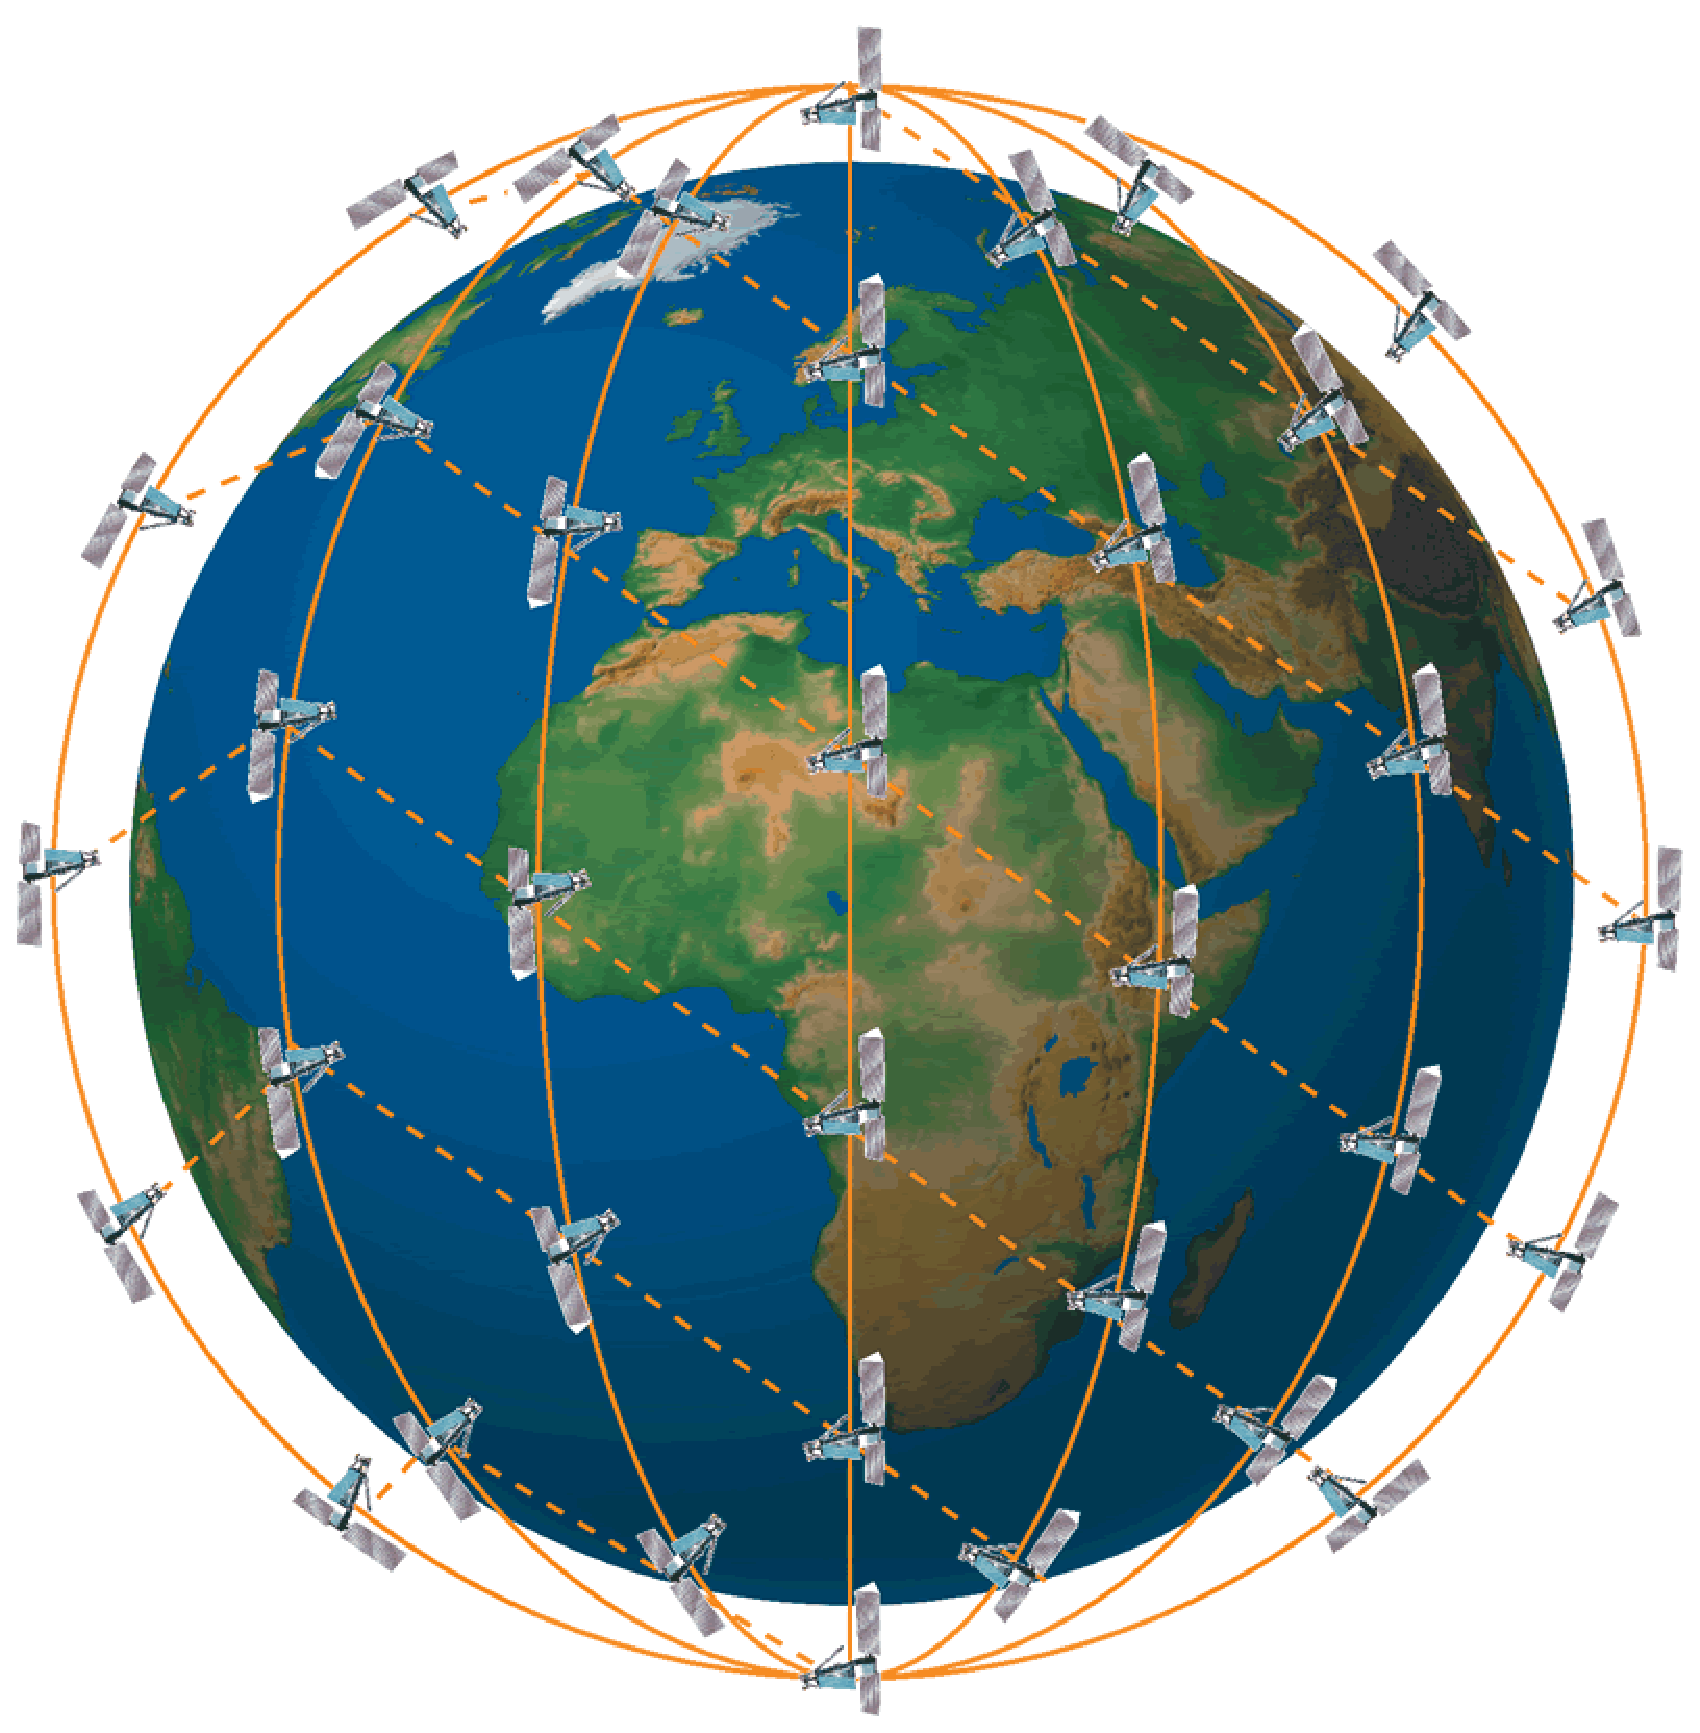
\includegraphics[width=7cm]{pic/SPAC_Iridium_Constellation_III_lg.eps}
    \caption{第一代铱星星座系统\protect\footnotemark}
    \label{fig:SPAC_Iridium_Constellation_III_lg}
    \end{figure}

    \footnotetext{图片来源:\url{https://www.rvmobileinternet.com/satellite-internet-update-iridium-oneweb-spacex-and-hughesnet/}}

    \item \textbf{第二代铱星}

    2008 年 8 月,铱星选择了 Lockheed Martin 和 Thales Alenia Space 两家公司参与下一代卫星星座的采购竞标。2010 年 6 月,该合同的获胜者为 Thales Alenia Space。SpaceX 已经签约将会发射所有的 Iridium NEXT 卫星。Iridium NEXT 卫星如图\ref{fig:IMG_Iridium-Satellite_NEXT-Satellite-Vehicle}所示。

    \begin{figure}[!htb]
    \centering
    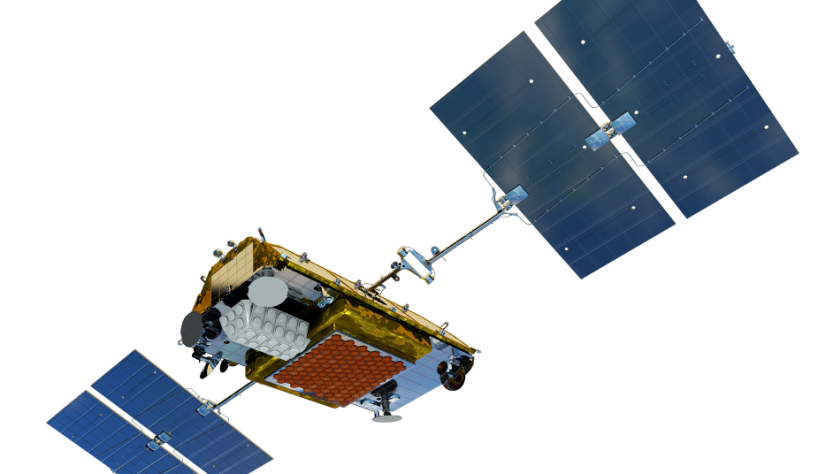
\includegraphics[width=13cm]{pic/IMG_Iridium-Satellite_NEXT-Satellite-Vehicle_HR_FEB16-clip-833x474.png}
    \caption{第二代铱星卫星}
    \label{fig:IMG_Iridium-Satellite_NEXT-Satellite-Vehicle}
    \end{figure}

    \renewcommand\arraystretch{1.5}
    \begin{table}[!htb]
    \centering
    \caption{第二代铱星卫星基本参数}
    \label{tab:iridium_next_paras}
    \begin{tabular}[b]{|p{4cm}<{\raggedleft}|p{8cm}<{\raggedright}|}
    \hline
    \textbf{帆板展开后翼展} & 9.4m \\
    \hline
    \textbf{卫星质量} & 约 860kg\\
    \hline
    \textbf{帆板收起时尺寸}& 3.1m x 2.4m x 1.5m \\
    \hline
    \textbf{轨道} & 圆极轨道(低地球轨道,LEO),海拔 780 km,倾角 86.4$^\circ$,周期 101 分钟,运行速度 24000 km/h(所有卫星总共分布于 6 个轨道上,每条轨道上包含 11 颗卫星)\\
    \hline
    \end{tabular}
    \end{table}

    2017 年 1 月,第二代铱星(Iridium NEXT)卫星开始部署到现有的星座中,Iridium SSC 的继承公司铱星通信公司(Iridium Communications)已经订购了由 Thales Alenia Space 和 Orbital ATK 共建造的共 81 颗新卫星,包括 66 颗在轨卫星,9 颗在轨备用卫星和 6 颗地面备用卫星。

    2017 年 1 月 14 日,第一批共 10 颗 Iridium NEXT 卫星发射成功,标志着该星座部署正式开始。最近的一次发射在 2019 年 1 月 11 日完成,SpaceX 的猎鹰 9 火箭将最后 10 颗卫星送入轨道,将 Iridium NEXT 星座数量增加到 75 颗(66 颗在轨卫星 + 9 颗在轨备用卫星),标志着 Iridium NEXT 星座部署正式完成。

    Iridium NEXT 卫星提供了 L 波段高达 128 kbit/s 的移动终端数据传输速度,高达 1.5 Mbit/s 的航海终端数据传输速度,用于固定/可移动终端的 Ka-Band 数据传输速度高达 8 Mbit/s,可以提供机上 WiFi 服务。

    Iridium NEXT 为 Aireon 提供了二级载荷,是一个 ADS-B 接收器,并通过 FlightAware 软件由航空公司和空管使用,ADS-B 接收器原型如图\ref{fig:Appstar_with_Base}所示,接收器在卫星上的搭载位置如图\ref{fig:reconfigurable_multimission_payloads}所示。58 颗卫星上的三级载荷是加拿大 exactEarth 公司的海洋 \acs{AIS} 船舶跟踪接收器。Iridium NEXT 还提供与太空中其他卫星的数据链接。\upcite{h3}

    \begin{figure}[!htb]
    \centering
    \begin{minipage}[t]{0.48\textwidth}
    \centering
    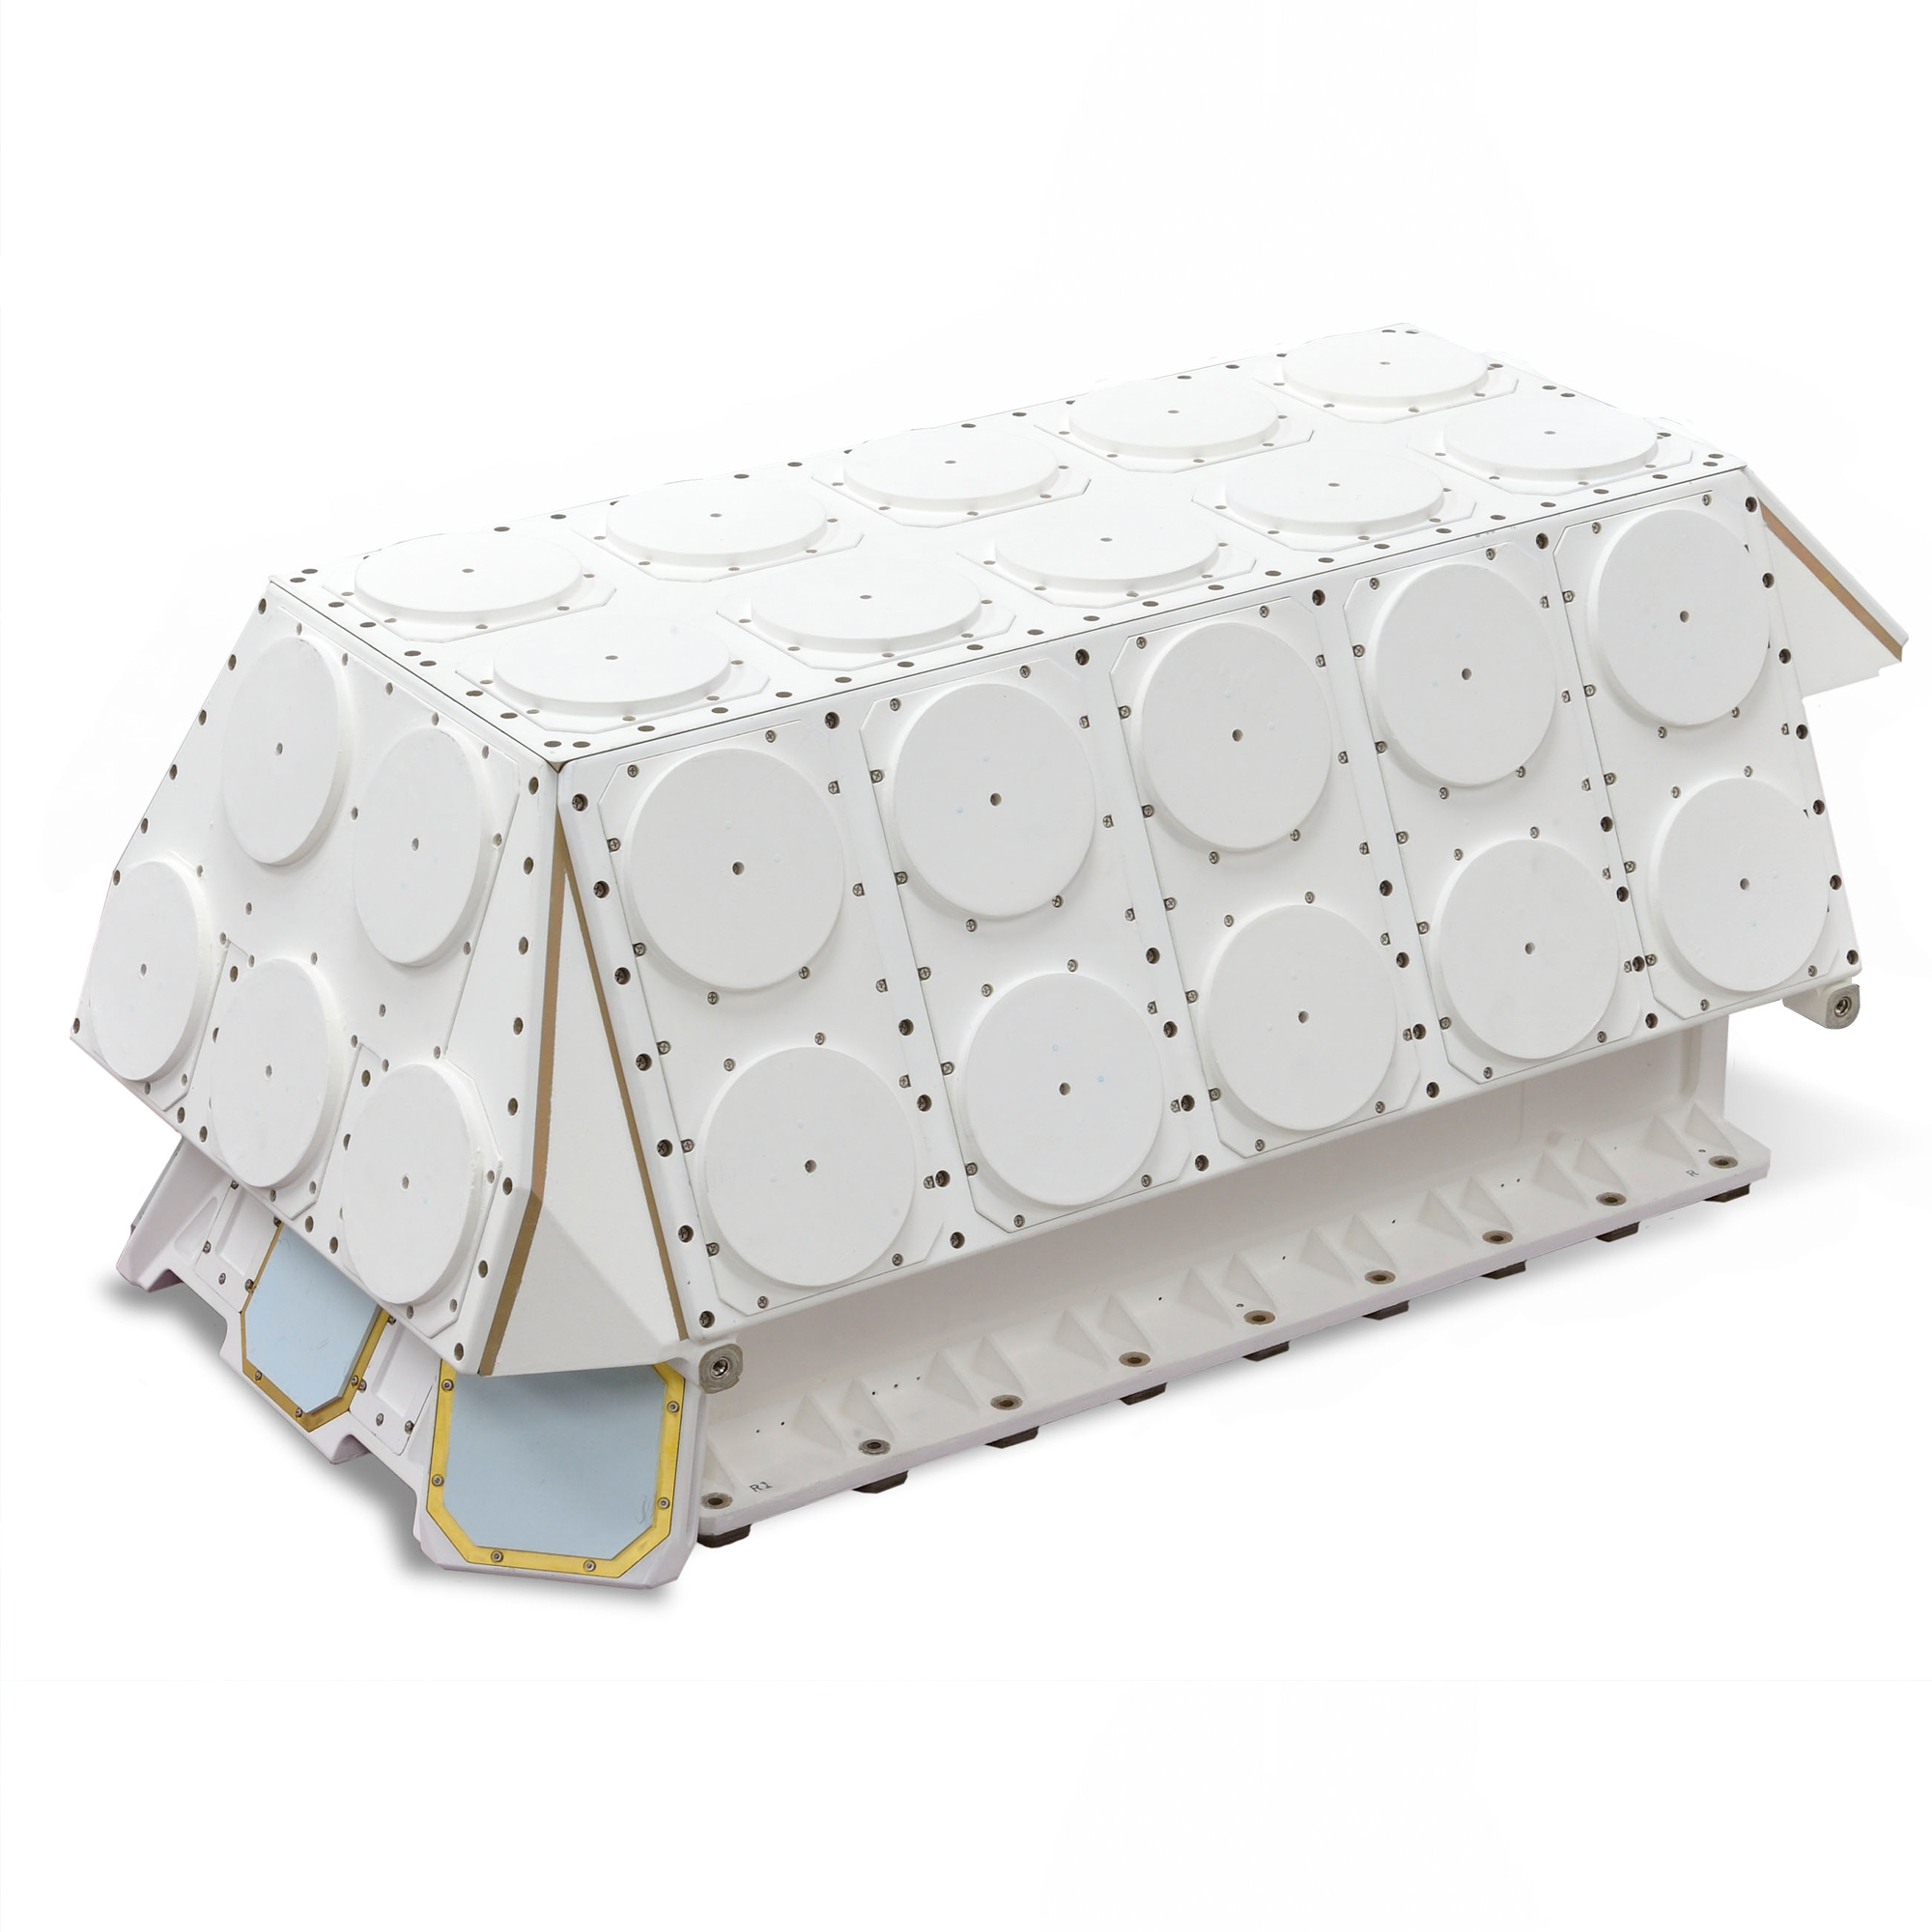
\includegraphics[width=6.5cm]{pic/Appstar_with_Base_2000x2000.jpg}
    \caption{Iridium NEXT 上的 ADS-B 接收器\protect\footnotemark}
    \label{fig:Appstar_with_Base}\footnotetext{图片来源:\url{https://www.harris.com/solution/reconfigurable-multimission-payloads}}
    \end{minipage}
    \begin{minipage}[t]{0.48\textwidth}
    \centering
    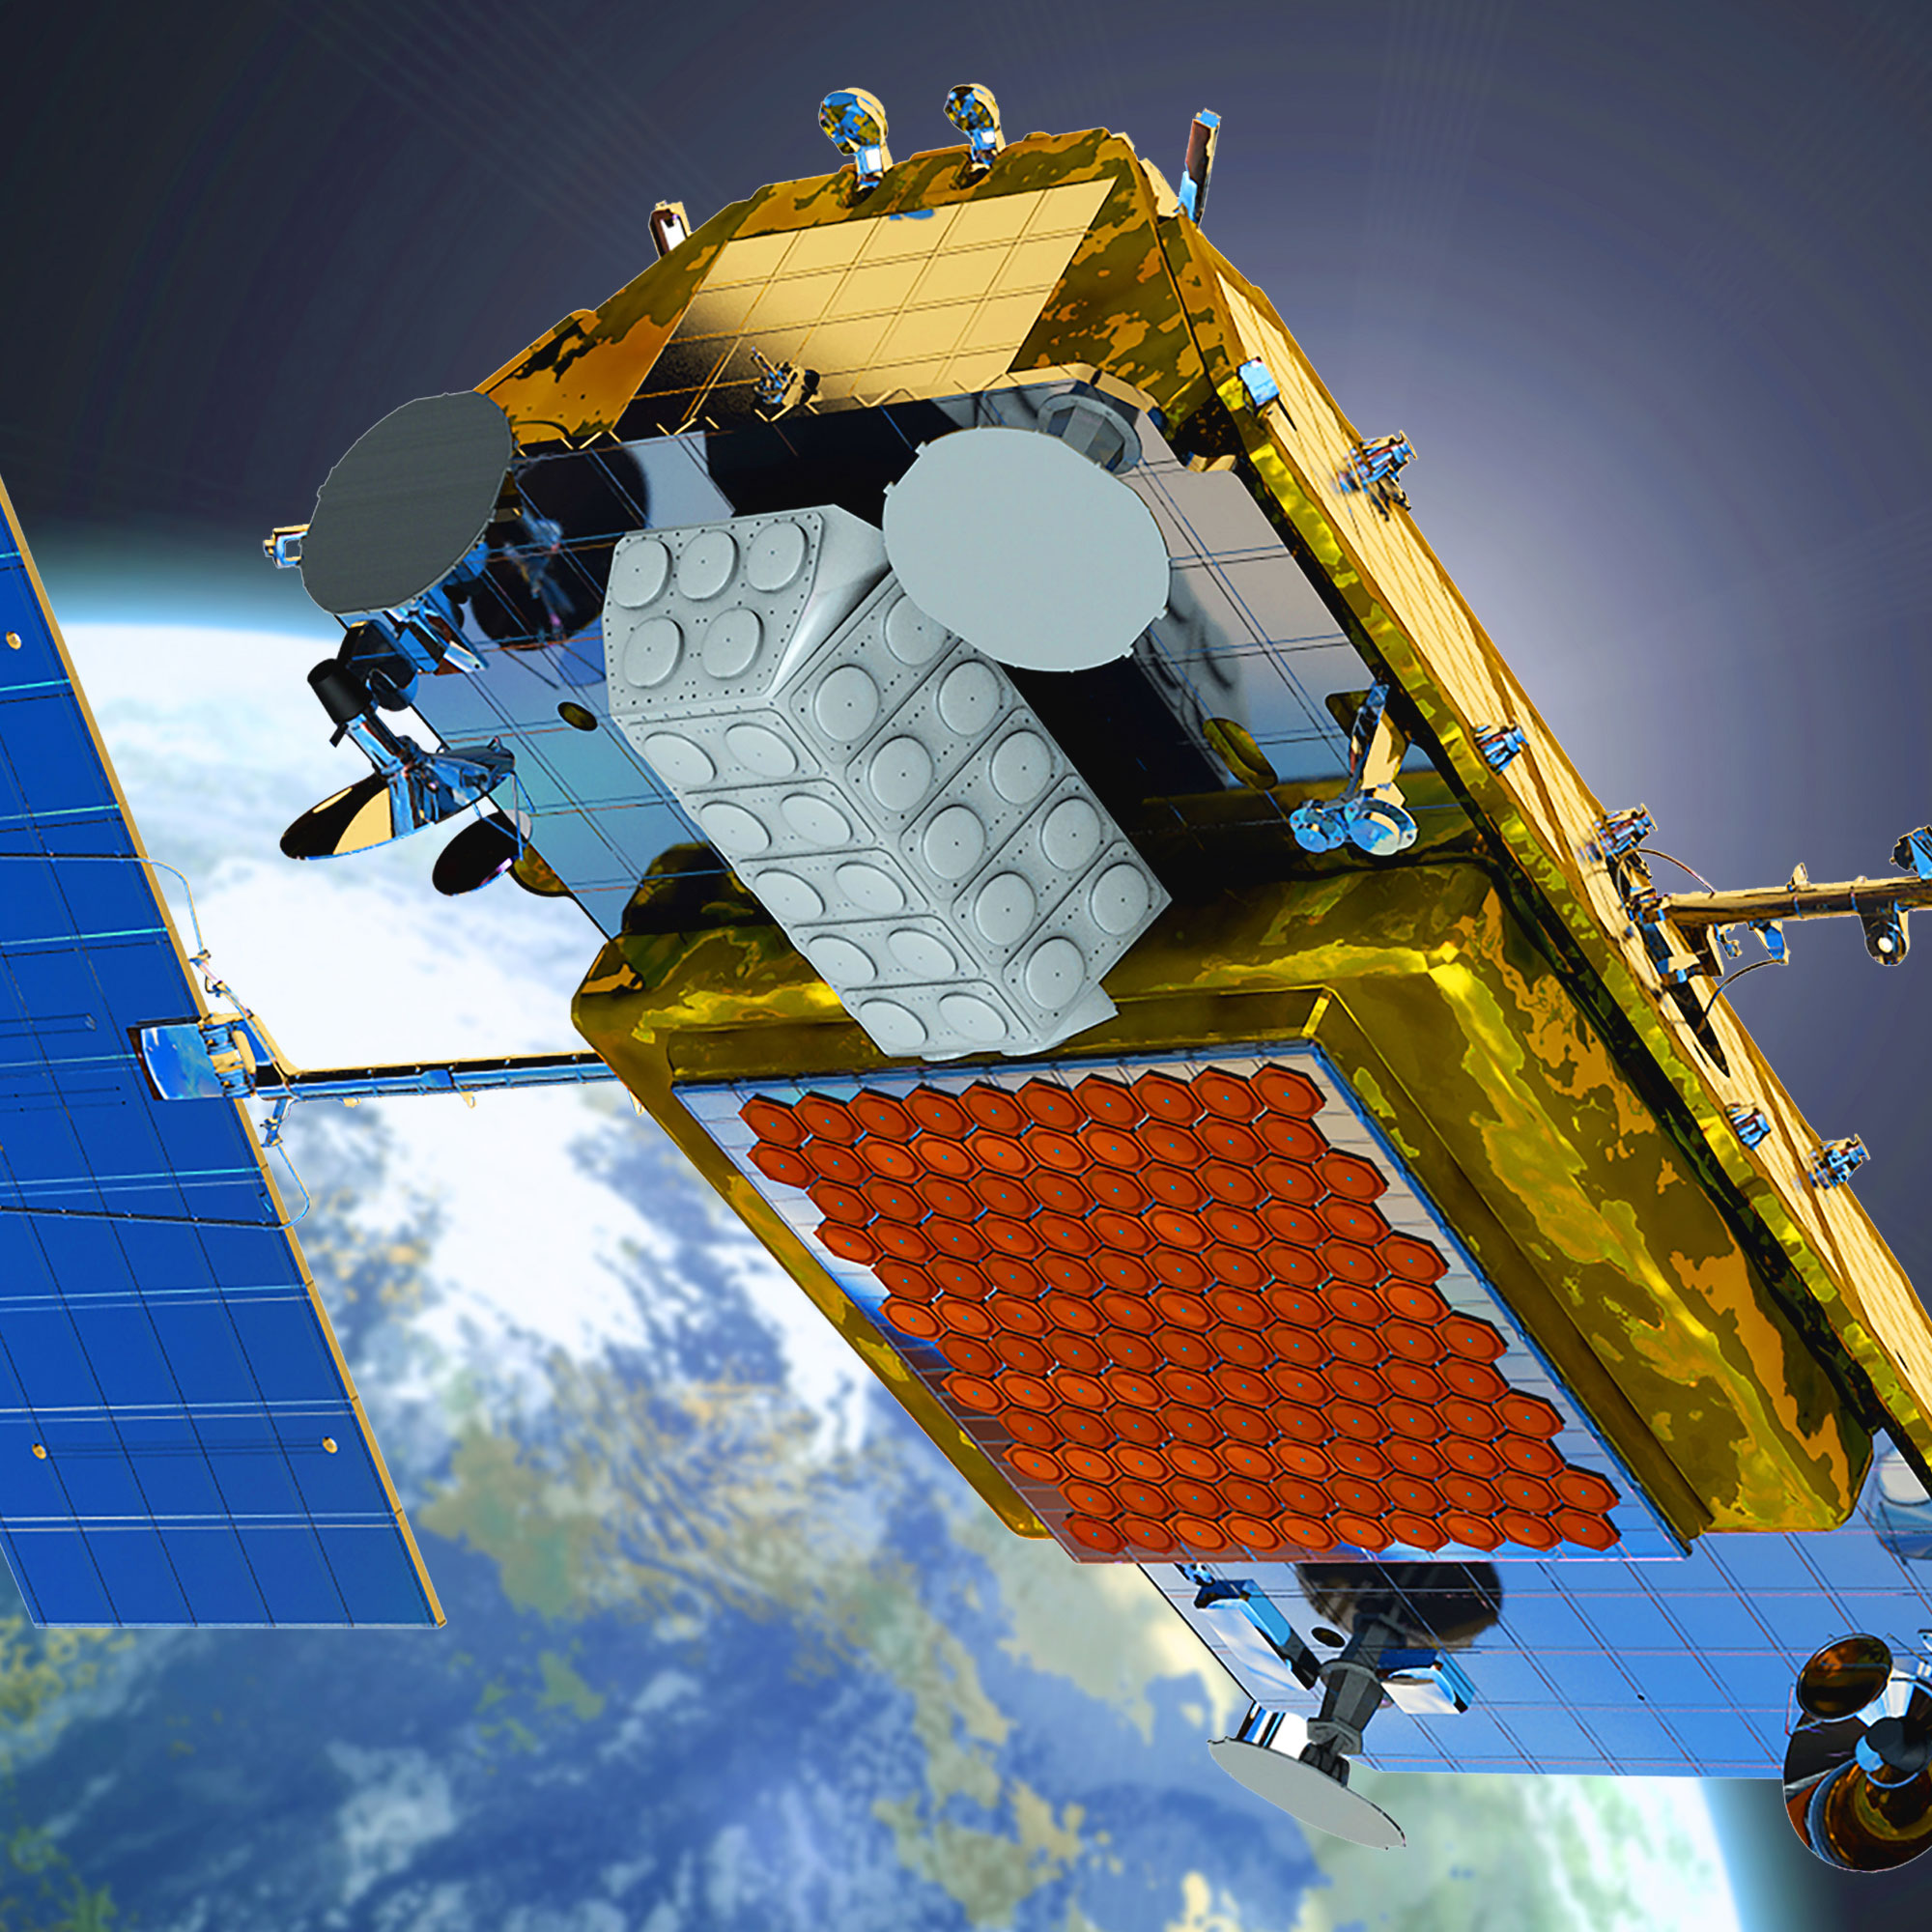
\includegraphics[width=6.5cm]{pic/reconfigurable_multimission_payloads_v2_web.jpg}
    \caption{ADS-B 接收器搭载方式\protect\footnotemark}
    \label{fig:reconfigurable_multimission_payloads}\footnotetext{图片来源:\url{https://www.harris.com/solution/reconfigurable-multimission-payloads}}
    \end{minipage}
    \end{figure}

\end{itemize}

\subsection{体系结构}

Aireon 的星基 ADS-B 系统布局原理如图\ref{fig:Aireon_GlobalSpaceBasedADSB_Coverage_Diagram}所示。

\begin{figure}[!htb]
\centering
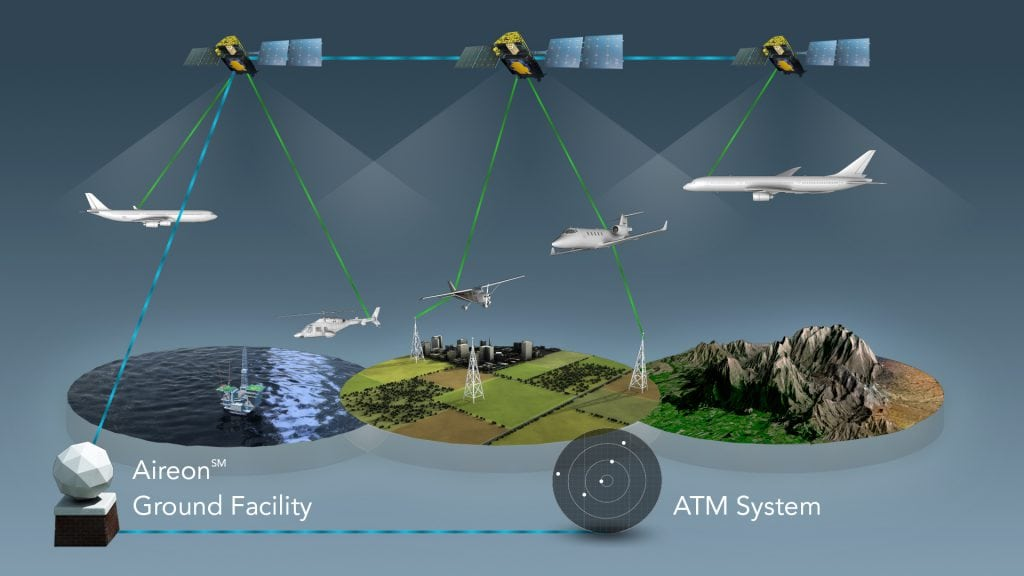
\includegraphics[width=14cm]{pic/Aireon_GlobalSpaceBasedADSB_Coverage_Diagram-1024x576.jpg}
\caption{Aireon 天基 ADS-B 系统布局原理\protect\footnotemark}
\label{fig:Aireon_GlobalSpaceBasedADSB_Coverage_Diagram}
\end{figure}

\footnotetext{图片来源:\url{https://www.aviationtoday.com/2018/01/19/space-based-ads-b-undergoes-successful-testing/}}

如图\ref{fig:System-Diagram-1024x693}所示,从飞机上广播的 ADS-B 信息将由 Harris 建造的有效载荷(AHP)接收,AHP 将接收到的数据在卫星之间互传,然后下行传至 Aireon 的地面传送网络(TPN)和 Aireon 的处理和分配系统(APD)。在合作伙伴 Harris 的帮助下,APD 对数据进行解码和验证,并将数据传递给购买了 Aireon 服务的客户。

\begin{figure}[!htb]
\centering
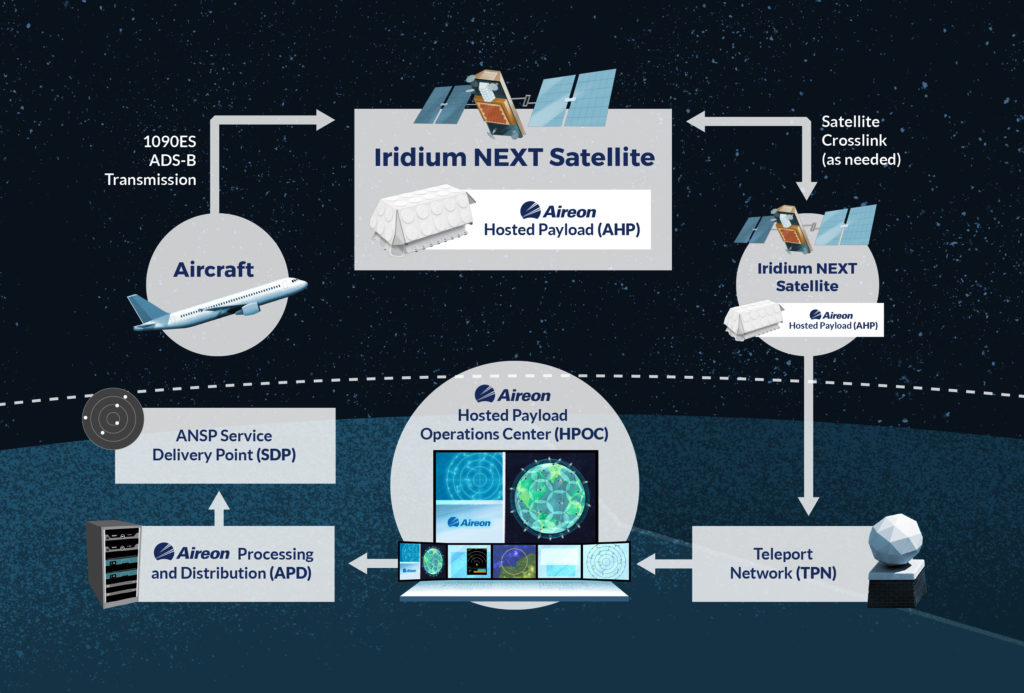
\includegraphics[width=13cm]{pic/System-Diagram-1024x693.jpg}
\caption{Aireon 天基 ADS-B 系统架构\protect\footnotemark}
\label{fig:System-Diagram-1024x693}
\end{figure}

\footnotetext{图片来源:参考文献\cite{e16}}

\subsection{系统性能}

Aireon 的星基 ADS-B 系统,目前只考虑了在卫星上安装 1090ES ADS-B 接收机,没有考虑安装 1090ES ADS-B 发射机。因此,该系统主要用于飞行监视和追踪,没有 \acs{TIS}/\acs{FIS} 上传能力\upcite{z1}。它的主要性能如表\ref{tab:aireon_ads-b_performance_para}所示。

\renewcommand\arraystretch{1.5}
\begin{table}[!htb]
\centering
\caption{Aireon 星基 ADS-B 系统的性能}
\label{tab:aireon_ads-b_performance_para}
\begin{tabular}[b]{|p{2.2cm}<{\raggedleft}|p{10.5cm}<{\raggedright}|}
\hline
\textbf{适用性} & 兼容所有符合 DO-260 标准的 1090ES ADS-B 设备 \\
\hline
\textbf{覆盖范围} & 可实现全球范围内不间断的覆盖 \\
\hline
\textbf{可用性} & 大于 99.9\% \\
\hline
\textbf{容量} & 每个点波束 1000 架飞机 \\
\hline
\textbf{时延} & ATC 检测追踪小于 1.5s \\
\hline
\textbf{更新速率} & 95\% 的响应速度小于 8s \\
\hline
\textbf{部署} & 已经部署完毕,2018 年 9 月提供全球的星基 ADS-B 服务 \\
\hline
\textbf{平均寿命} & 14 年 \\
\hline
\end{tabular}
\end{table}

根据 Aireon 的资料显示,Aireon 的星基 ADS-B 系统卫星组网后的覆盖范围虽然可以覆盖全球,但是其覆盖范围也会受许多因素影响,其中航空电子设备标准确定了功率输出为 125 瓦、250 瓦和 500 瓦的机载发射机的等级,图\ref{fig:CPWG16_PPT09_Satellite_Based_ADSB_December2013}和图\ref{fig:CPWG16_PPT09_Satellite_Based_ADSB_December2013_1}分别展示了 125 瓦发射机和 250 瓦发射机下的全球卫星组网覆盖范围。


\begin{figure}[!htb]
\centering
\begin{minipage}[t]{0.48\textwidth}
\centering
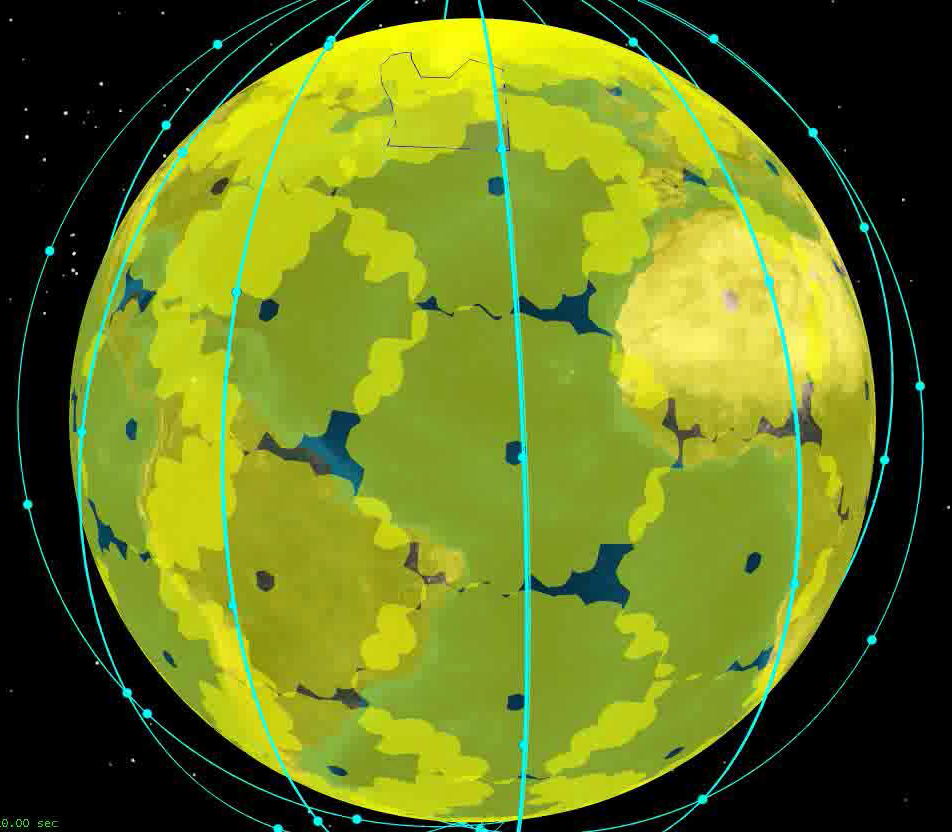
\includegraphics[height=6cm]{pic/CPWG16_PPT09_Satellite_Based_ADSB_December2013.png}
\caption{125W 功率下的全球覆盖范围\protect\footnotemark}
\label{fig:CPWG16_PPT09_Satellite_Based_ADSB_December2013}\footnotetext{图片来源:参考文献\cite{e13}}
\end{minipage}
\begin{minipage}[t]{0.48\textwidth}
\centering
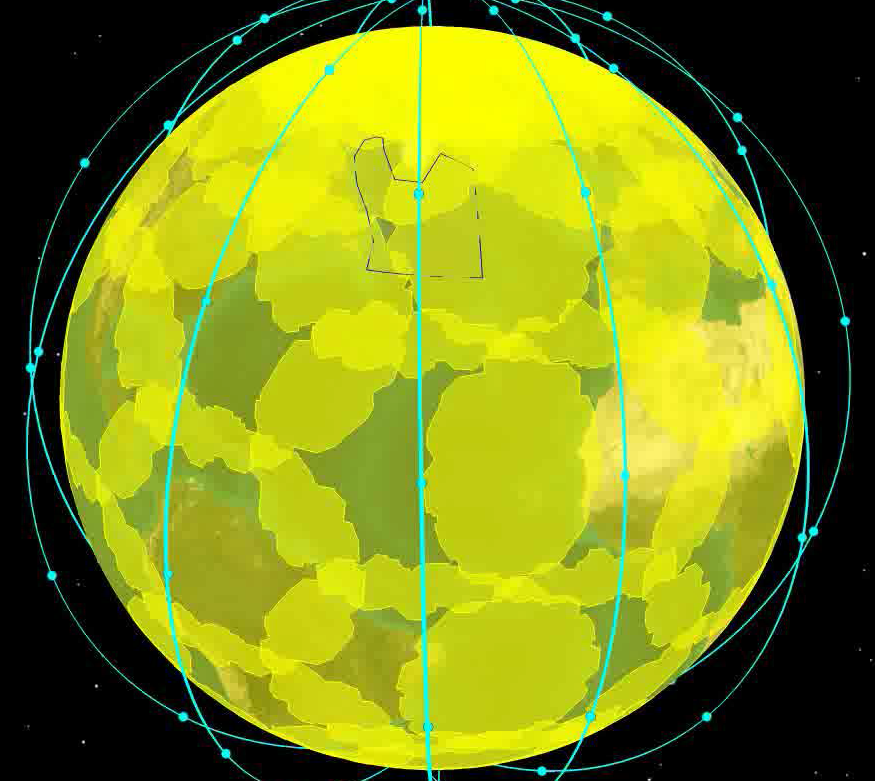
\includegraphics[height=6cm]{pic/CPWG16_PPT09_Satellite_Based_ADSB_December2013_1.png
}
\caption{250W 功率下的全球覆盖范围\protect\footnotemark}
\label{fig:CPWG16_PPT09_Satellite_Based_ADSB_December2013_1}\footnotetext{图片来源:参考文献\cite{e13}}
\end{minipage}
\end{figure}

Aireon 的星基 ADS-B 的卫星组网后每个卫星的覆盖范围互相重叠,组成了三角冗余区域,如图\ref{fig:Aireon-NAM-CAR-SAM-ADS-B-WS-v4-31}所示。

\begin{figure}[!htb]
\centering
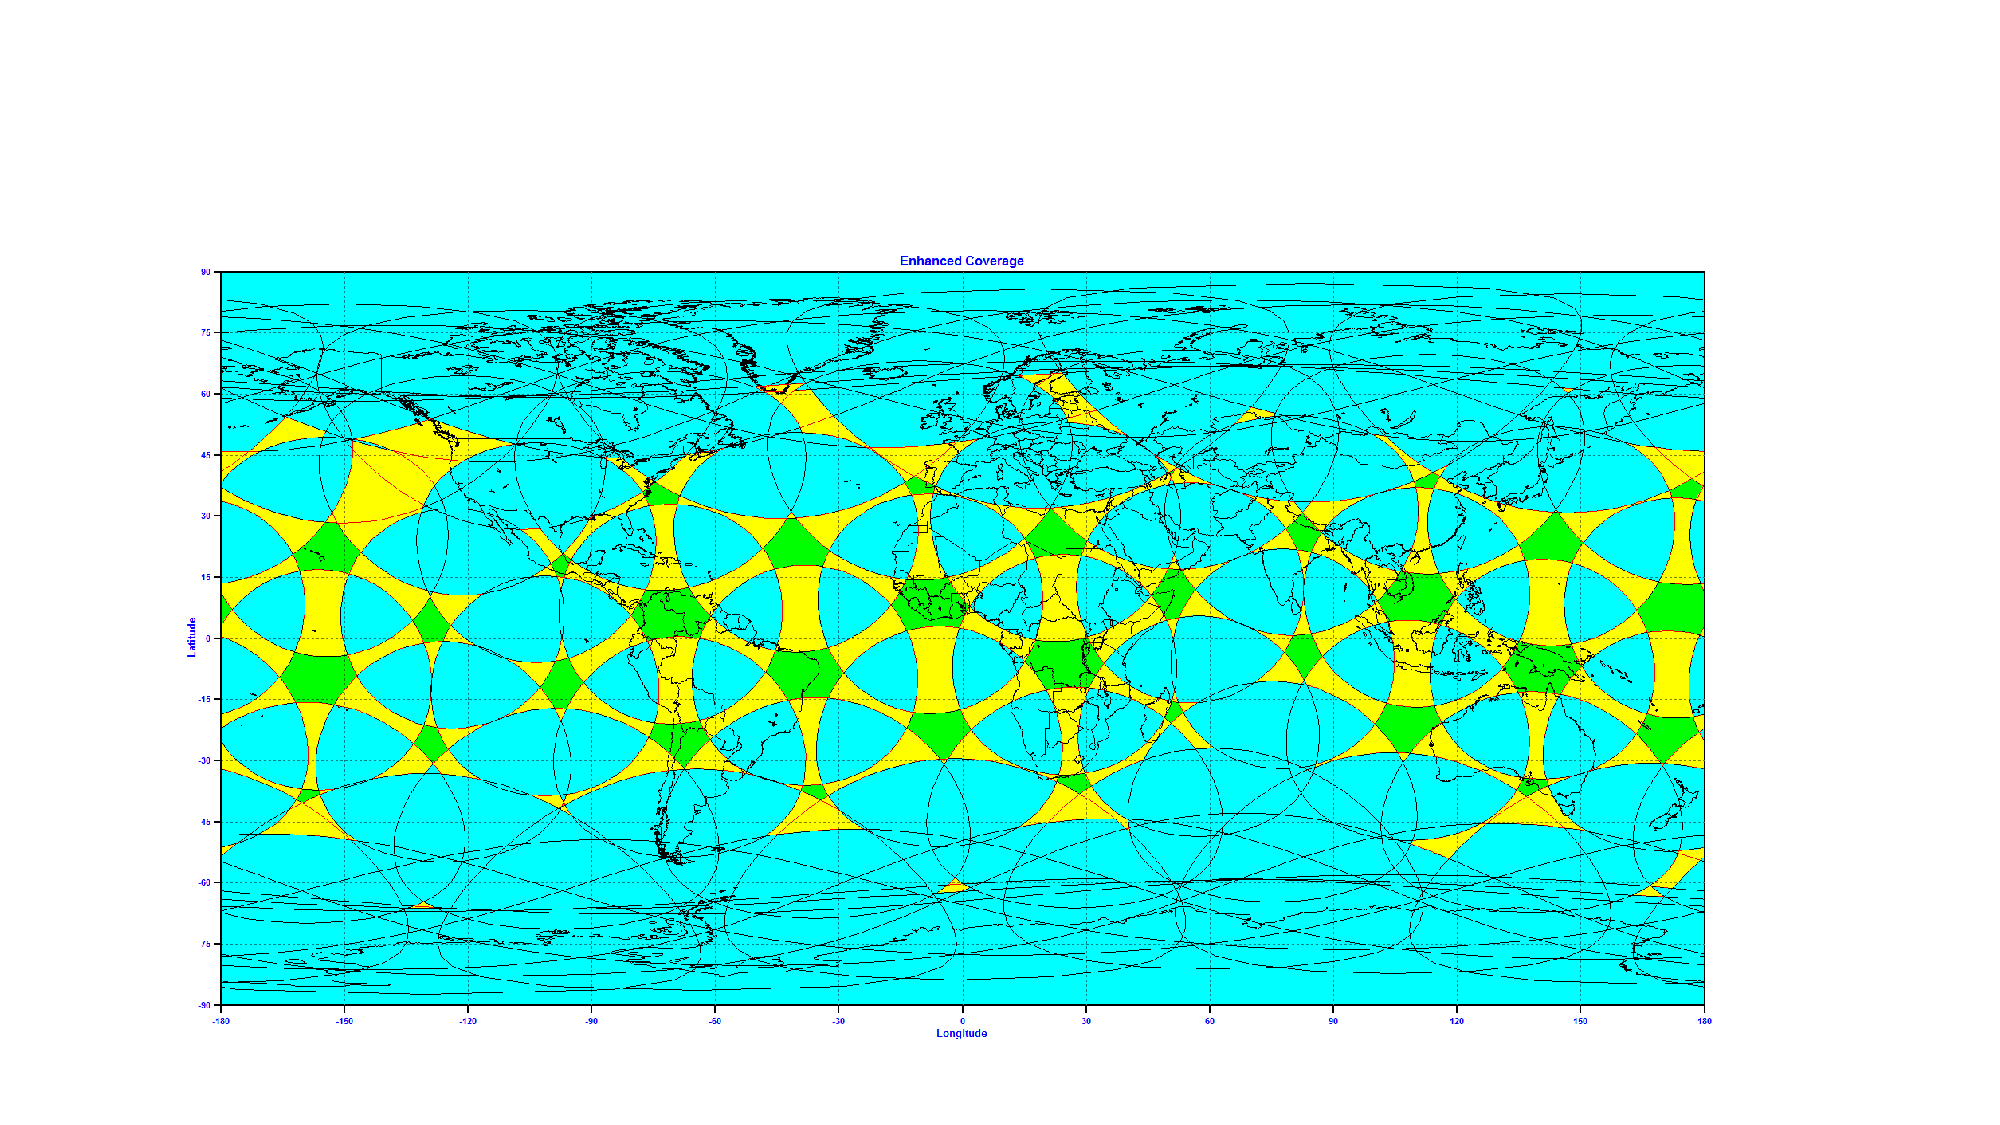
\includegraphics[width=14.5cm]{pic/Aireon-NAM-CAR-SAM-ADS-B-WS-v4-31.pdf}
\caption{Aireon 的星基 ADS-B 覆盖三角冗余区域\protect\footnotemark}
\label{fig:Aireon-NAM-CAR-SAM-ADS-B-WS-v4-31}
\end{figure}

\footnotetext{图片来源:参考文献\cite{e12}}

\subsection{系统评价}

目前 Aireon 的星基 ADS-B 系统已经基本部署完成,Iridium NEXT 星座部署已经全部完成,NAV CANADA、NAVAIR、IAA 和 CAAS 等一些地区 ANSP 已经开始体验 Aireon 的星基 ADS-B 服务,并且该系统的免费 ALERT 服务也已经上线,供全球航空相关的利益攸关方免费使用。

\section{ALAS 系统}

\subsection{系统概述}

ADS-B Technologies 公司推出了另一款基于卫星的 ADS-B 产品,该公司与 Globalstar 公司合作,借助 Globalstar 的卫星星座系统,将 ADS-B 模块融合到 Globalstar 的卫星上,提供全球 ADS-B 服务。该公司将天基 ADS-B 系统称为 ADS-B 链路增强系统(ADS-B Link Augmentation System),简称为“ALAS”。通过该系统,地球上任何地方的任意一架飞机可以被实时地安全追踪。

2010 年 5 月 16 日,ADS-B Technologies 公司在官网上发布推出 ALAS 系统的声明,并声明 ALAS 系统的一个重要特征是它可以作为外围设备使用,因此几乎可与任何 ADS-B 航空电子设备或地面收发器系统兼容。同时声称该系统已进行了三年多的开发和空中测试,Globalstar,Inc. 将为该技术提供卫星骨干网,评估单元应在 2011 年第 4 季度之前提供。

2011 年 7 月 22 日,ADS-B Technologies 公司在官网上发布声明声称为了帮助实现 NextGen 空中交通管理议程,ADS-B Technologies LLC 与 Globalstar, Inc. 合作开发了一个全球领先的卫星空中交通管制系统。并同时宣布 2011 年 7 月 13 日,使用联盟号运载火箭从哈萨克斯坦的拜科努尔航天发射场成功发射了 6 颗新的第二代全球星卫星。ADS-B Technologies 与 Globalstar,Inc. 签署了为期 10 年的正式协议,该协议于 2011 年 5 月 10 日宣布将在 Globalstar 的第二代卫星上使用其专有的 ADS-B 链路增强系统 ALAS 技术。

2011 年 12 月 28 日,ADS Technologies 宣布最近回应了美国联邦航空局的一项调查要求,该要求将确定能够在 2018 年开始为美国和海洋地区的偏远山区提供基于空间的自动相关监视 ADS-B 服务。这些系统将增强 FAA 国内地面 ADS-B 基础设施,最早将于 2013 年投入运营,并于 2020 年全面实施。2011 年 12 月 28 日,使用联盟号运载火箭从哈萨克斯坦的拜科努尔航天发射场成功发射了 6 颗第二代全球星卫星。ADS-B Technologies 公司总裁 Skip Nelson 说:“这意味着 Globalstar 现在已经实现了四分之三的目标,即推出 24 个新的高速,高容量卫星,能够支持我们基于 NextGen 空间的空中交通管理系统。”。“这也意味着,如果美国联邦航空局或任何其他民航组织要求,我们将在2014年底之前进行全面的运营测试。”

2012 年 5 月 7 日,ADS-B Technologies 宣布使用 Globalstar 卫星网在阿拉斯加深山通道完成其革命性的基于空间的 ADS-B 空中交通管制监视系统的首次公开演示。在 4 月的第三周进行的测试最终证明,现在可以在任何高度和地球上任何地方的任何地形上进行高度准确,可靠和低延迟的监视。

2014 年 9 月 3 日,ADS-B Technologies 宣布完成 7000 nm 双链 ALAS 的公共飞行演示,演示于 8 月 19 日开始,从安克雷奇出发,并通过横跨海湾的一次低空试飞达到了顶峰。在墨西哥完成测试的飞机于 9 月 2 日返回其安克雷奇主场。该航班飞行超过 7000 英里,包括墨西哥湾的 1100 英里往返里程,从凤凰城直飞西雅图,并在阿拉斯加湾上空飞行。在飞行期间,ADS-B Technologies 的首席科学家兼 ALAS 的合作设计师 Mike Melum 不仅同时传输了 ADS-B 链路上的低延迟 1 秒报告,还演示了实时 Globalstar SAT-FI 互联网和 Satcom 语音连接飞机 还携带了两个低成本的 Globalstar SPOT 单工跟踪设备,并有效地证明了它们能够为整个 7000 nm 行程提供无缝且非常精确的 2.5 分钟和 5 分钟位置报告。

\begin{figure}[!htb]
\centering
\begin{minipage}[t]{0.42\textwidth}
\centering
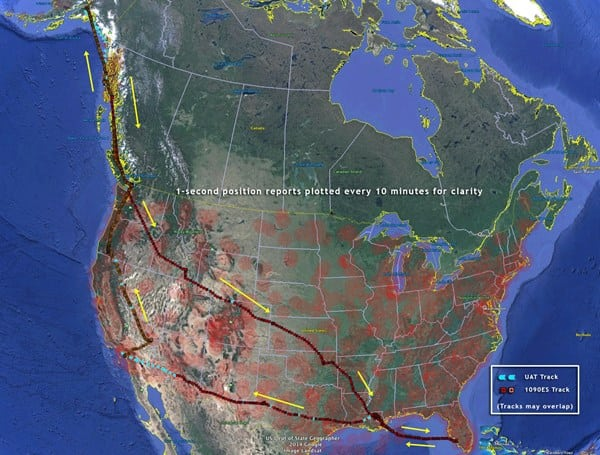
\includegraphics[width=6cm]{pic/311182-2.jpg}
\caption{ALAS 系统的飞行演示\protect\footnotemark}
\label{fig:311182-2}\footnotetext{图片来源:参考文献\cite{h12}}
\end{minipage}
\begin{minipage}[t]{0.56\textwidth}
\centering
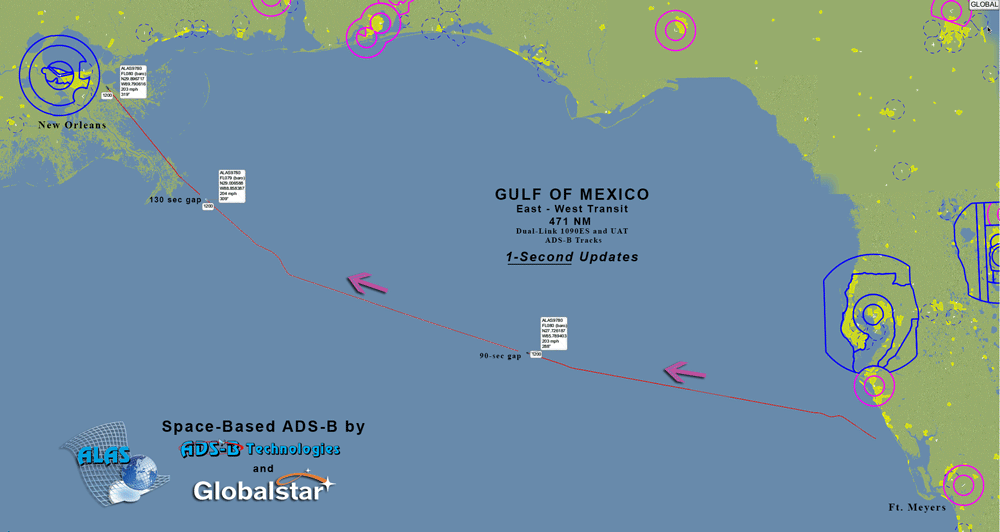
\includegraphics[width=8.5cm]{pic/GOM-L.png}
\caption{ALAS 系统墨西哥湾上空的飞行演示\protect\footnotemark}
\label{fig:GOM-L}\footnotetext{图片来源:参考文献\cite{h12}}
\end{minipage}
\end{figure}


2015 年 8 月 3 日,ADS-B Technologies 宣布完成其 ALAS 系统的另一次长途飞行演示,演示于 7 月 23 日在威斯康星州奥什科什举行的 2015 年 EAA AirVenture 飞行大会上。航班覆盖超过 5700 海里,包括加拿大西部和美国北部、落基山脉、西雅图和阿拉斯加东南部的最后一站,直到 7 月 30 日在安克雷奇的 ADS-B 技术基地降落。该航班再次证明 1090ES 和 UAT 基于空间的 ADS-B 在所有环境和长时间内都能很好地工作。ADS-B Technologies 的首席科学家 Mike Melum 评论说:“我们现在有超过 100 个飞行小时的 ALAS 性能数据。”

\begin{figure}[!htb]
\centering
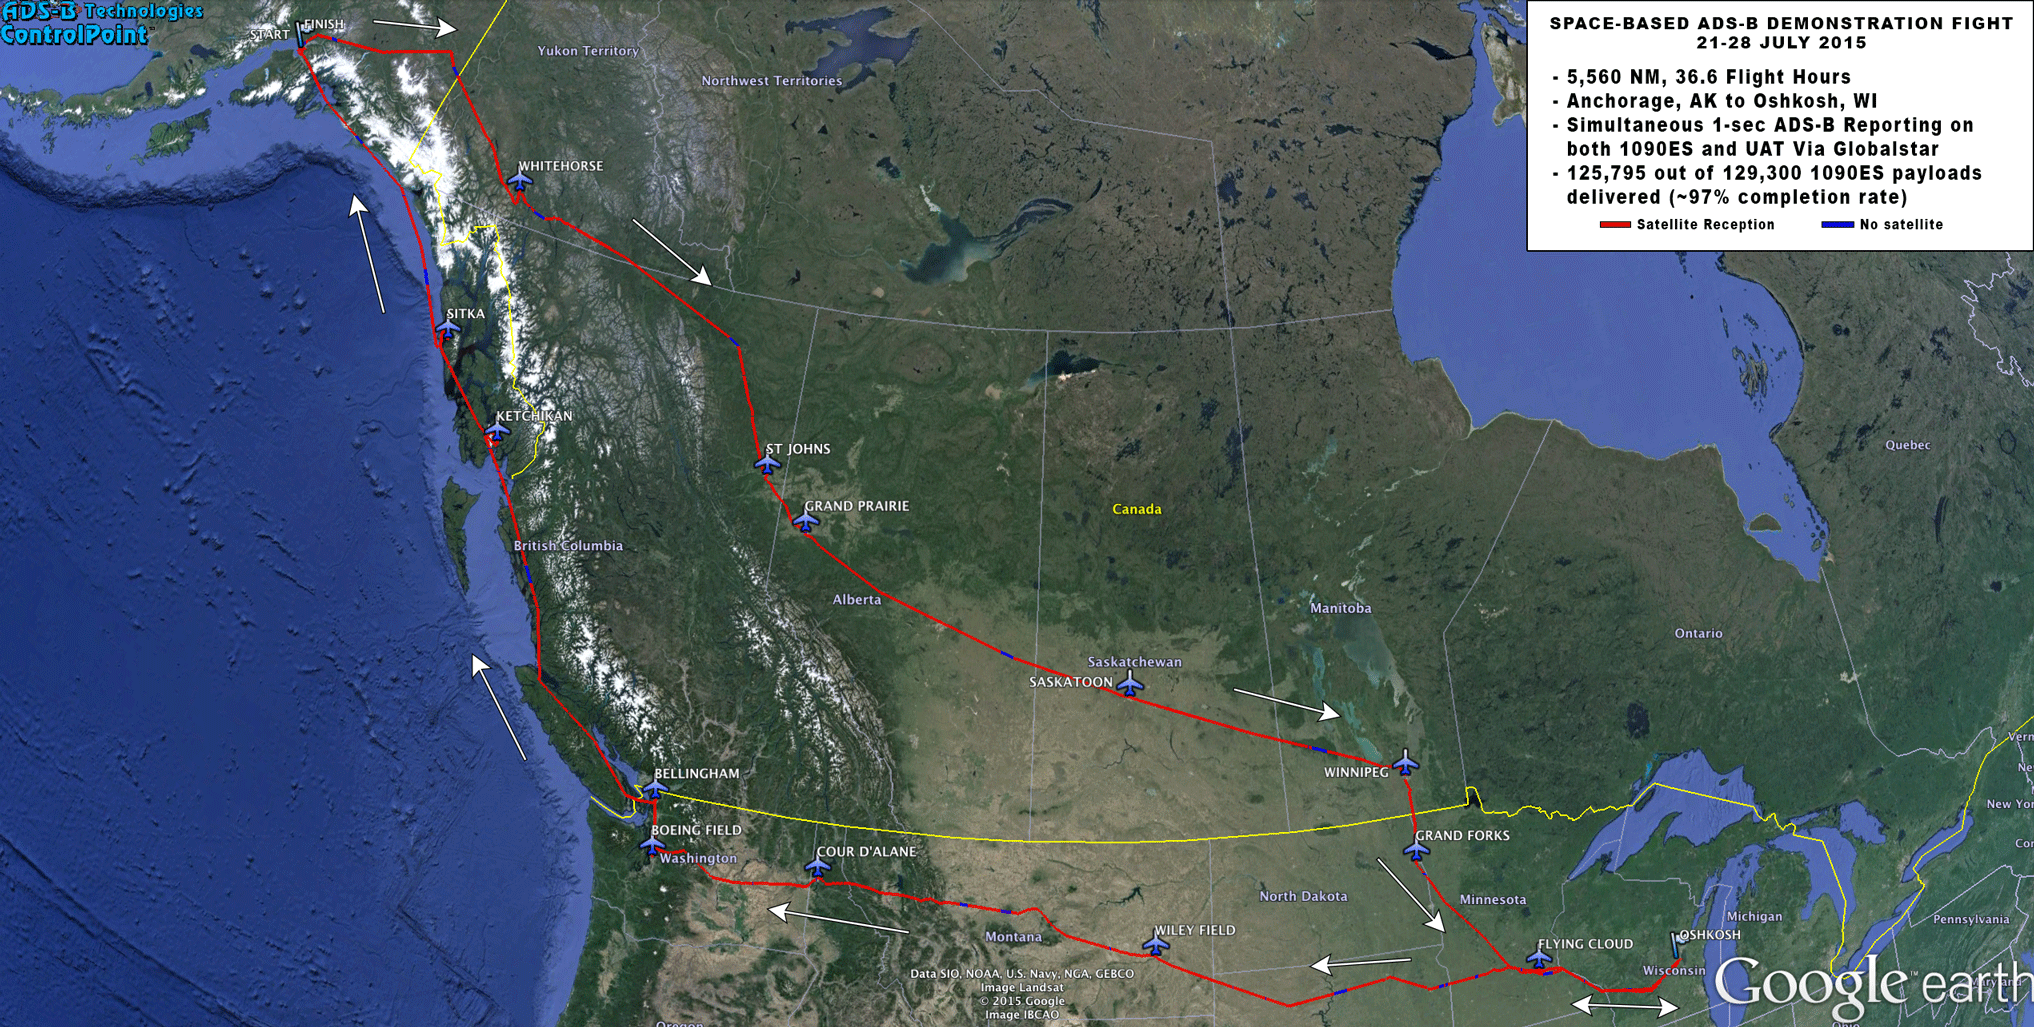
\includegraphics[width=14.5cm]{pic/Flight-Demo-21-July-15b.png}
\caption{ALAS 于 2015 年 7 月 21 日的飞行演示\protect\footnotemark}
\label{fig:Flight-Demo-21-July-15b}
\end{figure}

\footnotetext{图片来源:参考文献\cite{h12}}

2016 年 9 月 28 日,Globalstar 和 ADS-B Technologies 宣布完成 NASA 兰利研究中心研究飞行与 Cirrus SR22 无人机系统(UAS)代理设计测试 ALAS 的操作。初步结果表明飞机与 Globalstar 卫星系统之间的持续通信,在极端机动期间只有短暂的中断,并迅速重新连接。Cirrus SR22 测试飞行的重点是测试 ALAS 使用远程控制功能在飞机和 NASA 地面控制站之间连续传递双向数据的能力。两个 40 分钟飞行中的第一个包括极端机动,两个 60 度倾斜角度转弯专门用于测试 ALAS 连接。第二次飞行在一系列涉及航向和高度变化的机动过程中产生了类似的结果。“美国宇航局不仅证明 ALAS 在机动方面表现良好,而且还证实飞行控制命令,飞机状态和状态等复杂数据可以通过同一个强大的 Globalstar 链路实时传递给控制器​​,”ADS-B Technologies 总裁 Skip Nelson 说。“这告诉我们,ALAS 可以在飞机和地面之间提供单一,安全且可能加密的门户。”\upcite{h12}

\subsubsection{Globalstar 简介}

Globalstar,Inc. 是一家美国卫星通信公司,运营着用于卫星电话和低速数据通信的 LEO 卫星星座,有点类似于铱卫星星座和 Orbcomm 卫星系统。Globalstar 第二代星座由 24 颗 LEO 卫星组成。

Globalstar 项目于 1991 年成立,是 Loral Corporation 和 Qualcomm 的合资企业。1994 年 3 月 24 日,两家赞助商宣布成立 Globalstar LP,这是一家在美国成立的有限合资企业,其中包括阿尔卡特,AirTouch,德国航空,现代和沃达丰等八家公司的财务参与。当时,该公司预计该系统将于 1998 年推出,基于 18 亿美元的投资。

1995 年 1 月,Globalstar 从美国联邦通信委员会获得了美国的频谱划分,并继续与其他国家进行谈判,以获得在其国家使用相同无线电频率的权利。

第一批卫星于 1998 年 2 月发射,但由于 1998 年 9 月发射失败导致系统部署延迟,导致俄罗斯航天局在发射中丢失了 12 颗卫星。2000 年 2 月,它发射了 52 颗卫星中的最后一颗——第 48 颗卫星和 4 颗在轨备件。另外 8 颗未发射的卫星被保留为地面备件。

1999 年 10 月,该系统开始进行“友好用户”试验,共有 48 颗计划卫星中的 44 颗参与实验。1999 年 12 月,该系统开始为 200 名用户提供有限的商业服务,其中包括 48 颗卫星(轨道上没有备件参与)。2000 年 2 月,它在北美、欧洲和巴西开展了 48 颗卫星和 4 颗备件的全面商业服务,初始价格为每分钟 1.79 美元。

2002 年 2 月 15 日,Globalstar 前身公司(旧 Globalstar)及其三家子公司根据美国破产法第 11 章提交了自愿申请。

2004 年,旧 Globalstar 的重组工作已经完成。重组的第一阶段于 2003 年 12 月 5 日完成,当时 Thermo Capital Partners LLC 被视为获得业务的运营控制权,以及某些所有权和风险。Thermo Capital Partners 成为主要所有者。

Globalstar LLC 于 2003 年 11 月成立为特拉华州有限责任公司,并于 2006 年 3 月 17 日转为 Globalstar, Inc .。

2007 年,Globalstar 向太空发射了 8 颗第一代备用卫星,以帮助弥补其在轨卫星的过早失效。2010 年至 2013 年期间,Globalstar 发射了 24 颗第二代卫星,以恢复其全面服务系统。Globalstar 第二代卫星如图\ref{fig:globalstar-satellite}所示。

\begin{figure}[!htb]
\centering
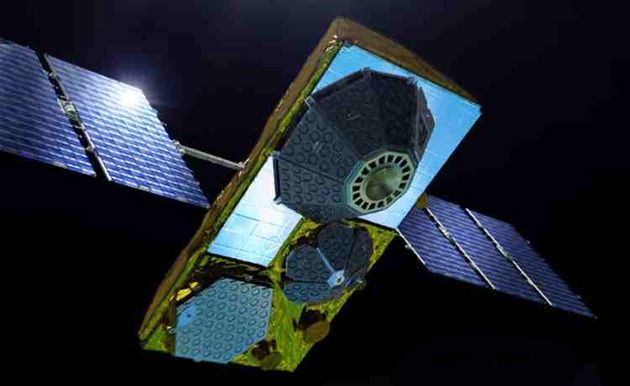
\includegraphics[width=10cm]{pic/globalstar-satellite.jpg}
\caption{Globalstar 第二代卫星\protect\footnotemark}
\label{fig:globalstar-satellite}
\end{figure}

\footnotetext{图片来源:\url{https://chinese.engadget.com/2014/01/30/globalstar-sat-fi/}}

2010 年至 2011 年间,Globalstar 将其总部从硅谷迁至路易斯安那州的卡温顿,部分原因是为了利用该州的税收优惠和低廉的生活成本。

2018 年 4 月,Globalstar 宣布将与 FiberLight 合并,交易价值 16.5 亿美元。\upcite{h11}

\subsection{体系结构}

ALAS 系统的体系结构如图\ref{fig:31-Globalstar-4}所示,其体系结构与 Aireon 的星基 ADS-B 系统相似,可以同时支持 1090ES 和 978UAT 数据链,但 ALAS 系统具备 TIS-B\footnote{TIS-B 是一种监视服务,称为交通信息服务广播,它从一个或多个基于雷达的监视源 ASDE-X 和 WAM 中获取交通信息,并将此交通信息上传到配备有 ADS-B 的飞机。TIS-B 使配备 ADS-B 的飞机能够接收到由雷达和上述系统监视到的非 ADS-B 飞机的位置报告。978UAT 和 1090ES 都支持 TIS-B 服务。}/FIS-B\footnote{FIS-B 是一种上行链路服务,提供天气以及其他航空信息(即 METAR、TAF、SIGMET、PIREP、NOTAM、NEXRAD、特殊用途空域状态等)。使用驾驶舱显示器,只有 978UAT 数据链支持 FIS-B 服务。} 上传能力,即卫星上不仅仅携带了 ADS-B 接收器,而且还可将相关信息转发给飞行器。TIS-B/FIS-B 上传服务使用卫星上的 S 波段天线转发。

\begin{figure}[!htb]
\centering
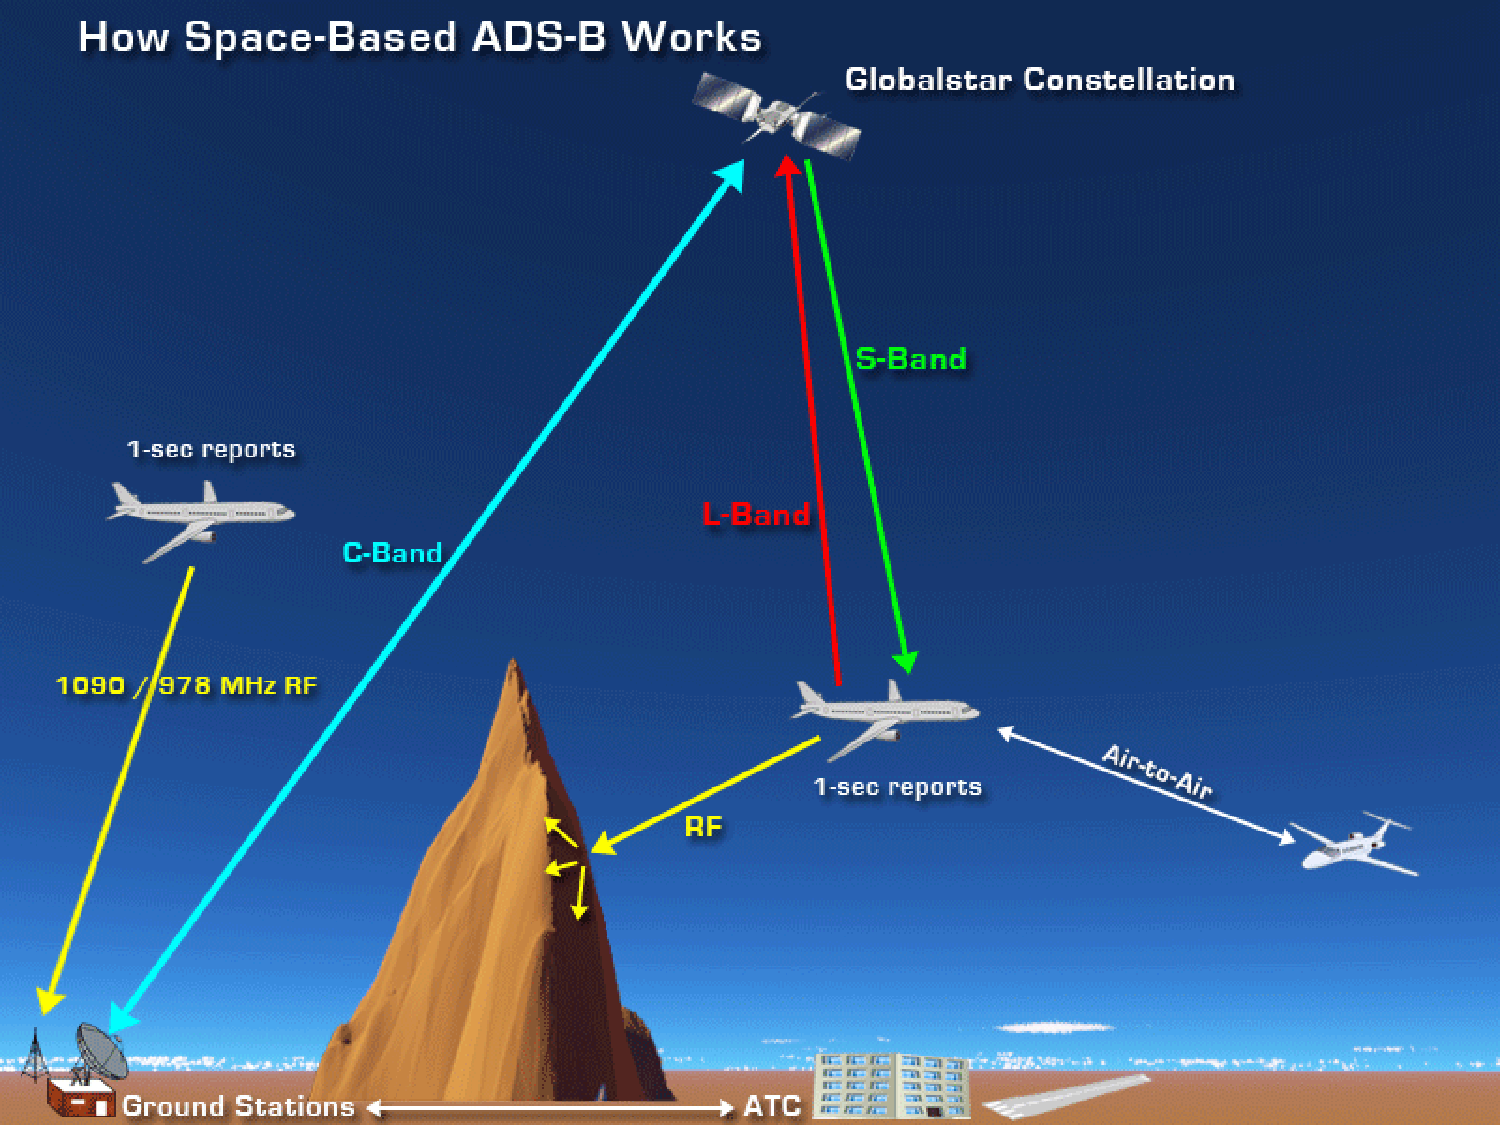
\includegraphics[width=14cm]{pic/31-Globalstar-4.pdf}
\caption{依托 Globalstar 的 ALAS 系统体系结构\protect\footnotemark}
\label{fig:31-Globalstar-4}
\end{figure}

\footnotetext{图片来源:参考文献\cite{e14}}

铱星系统和 Globalstar 系统不同点之一在于其卫星数据下行至地面的方式,铱星系统的原理是通过卫星间信道网络首先将需要下行的信息在卫星间通信传播,最后传到位于美国上空的卫星,通过该卫星将信息下传至美国的地面网关,再将信息通过美国的地面网关传输到其他节点。而 Globalstar 的做法是在全球各地设置网关,然后卫星网络直接将信息下行至世界各地的网关,然后直接经由世界各地的关口站将数据传送至各个节点,Globalstar 的体系结构在时延上要远远小于铱星系统。图\ref{fig:31-Globalstar-8}反映了全球星的双工网络通过 32 个地面网关覆盖了世界上 80\% 的重要航路。

\begin{figure}[!htb]
\centering
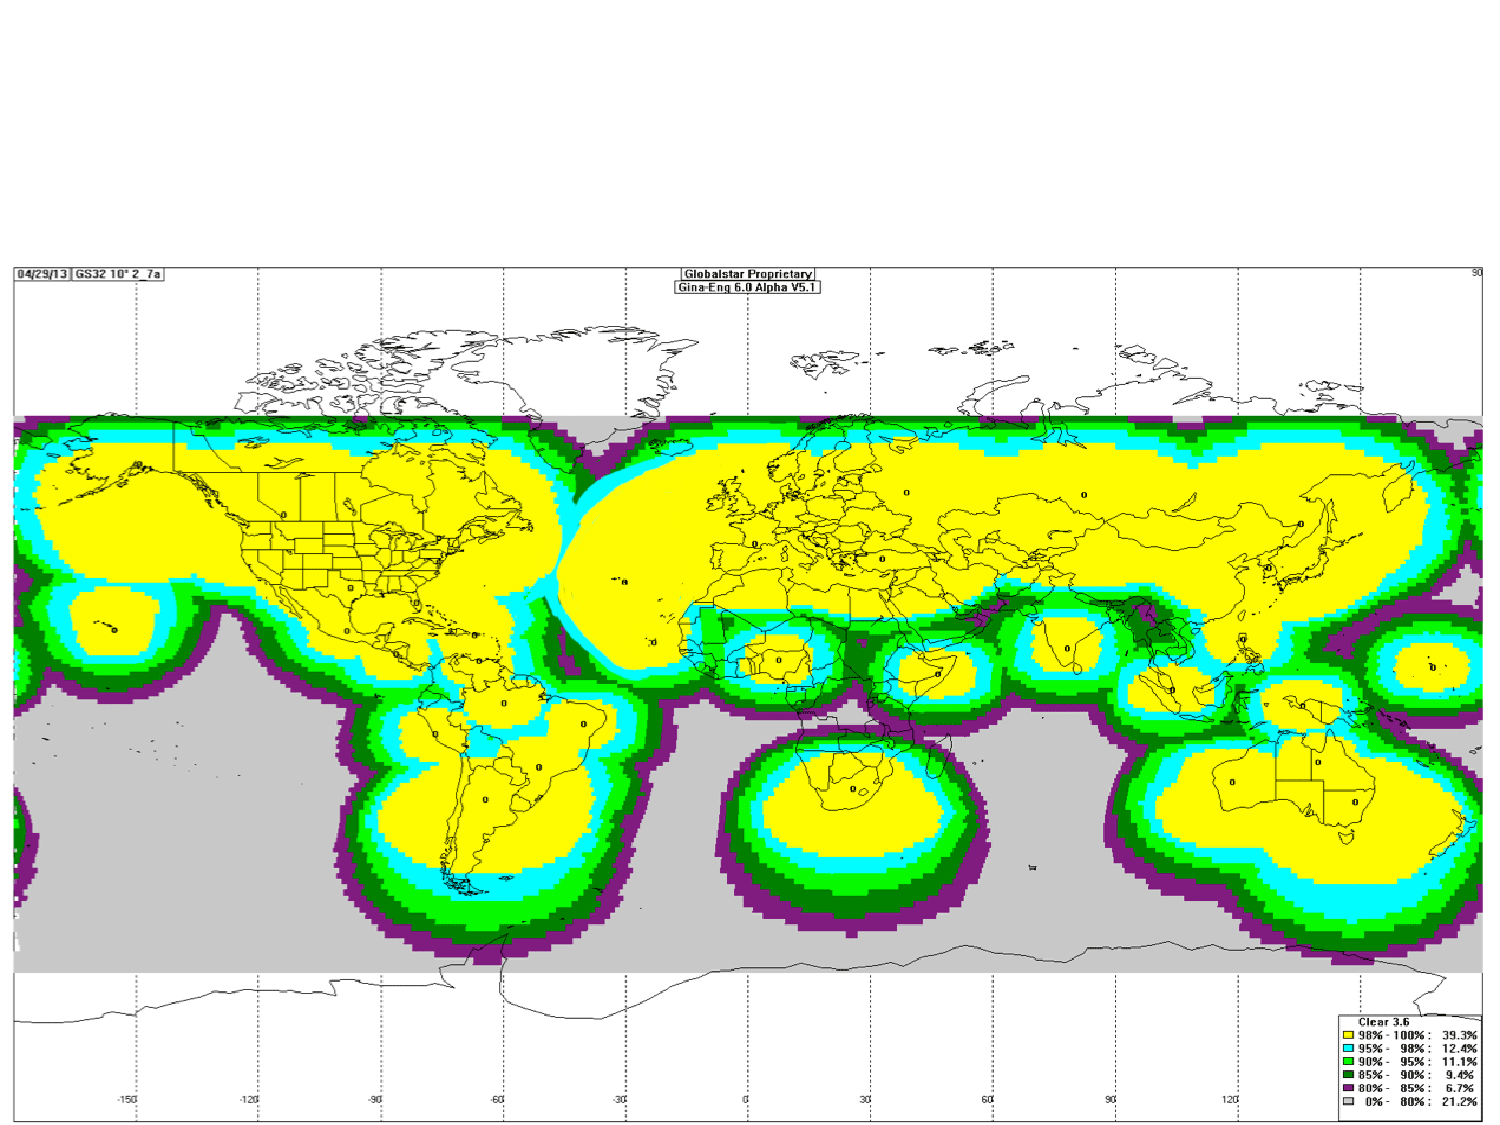
\includegraphics[width=15cm]{pic/31-Globalstar-8.pdf}
\caption{Globalstar 的双工网络全球覆盖范围\protect\footnotemark}
\label{fig:31-Globalstar-8}
\end{figure}

\footnotetext{图片来源:参考文献\cite{e14}}

\subsection{系统性能}

依托“全球星二代”系统的 ALAS 系统端到端(end-to-end)测试性能数据如表\ref{tab:alas-paras}所示。

\renewcommand\arraystretch{1.5}
\begin{table}[!htb]
\centering
\caption{使用全球星卫星的 ALAS 系统端到端测试性能\protect\footnotemark}
\label{tab:alas-paras}
\begin{tabular}[b]{|p{4cm}<{\raggedleft}|p{11cm}<{\raggedright}|}
\hline
\textbf{适用性
(Applicability)} &
ALAS 是一种简单、质量轻、低成本的外围设备,可与现有的任何 1090ES 或 UAT 电子设备配合使用,保证正常的空-地和地-空 ADS-B 传输不会中断。ALAS 还旨在与任何国家现有的 ADS-B 地面基础设施兼容\\
\hline
\textbf{覆盖范围(
Coverage Area)} &
到 2016 年,100\% 覆盖美国本土(CONUS)、GOMEX、加勒比海(Caribbean)、北大西洋(NAT)和北太平洋(NOPAC);到 2019 年,100\% 覆盖剩余地区\\
\hline
\textbf{可用性(
Availability)} & 到 2016 年,可用性为 99.99\%;到 2019 年,可用性为 99.999\% \\
\hline
\textbf{容量(
Capacity) }& 每架卫星可容纳大于 3000 架飞机(approx 1,800sm diameter)\\
\hline
\textbf{时延(
Latency)} &  从飞机到地面小于 200 毫秒;从端到端小于 300 毫秒 \\
\hline
\textbf{更新率(
Update Rate)} & 1 秒 \\
\hline
\textbf{完整性(
Integrity)} & 10E-6 \\
\hline
\textbf{精度(
Accuracy)} &
UTC 时制下,在 98\% 的时间里,相同目标的 射频视距(RF line-of-sight)导出位置和天基 ALAS 导出位置之间的显示位置差异小于 50 英尺\\
\hline
\textbf{安全性(
Security)} & 独一无二的安全。ALAS 与每架飞机建立了独特的双向连接,可以抵抗入侵、干扰或欺骗,是唯一的可以轻松加密的 ADS-B 形式。简单的防篡改设计还可以包括一个自供电备用系统,该系统将在未经授权而关闭飞机的主 ADS-B 转发器的情况下继续广播飞机的位置 \\
\hline
\textbf{可扩展性(
Scalability)}  & 高。系统架构的成本相对较低且简单,通过增加更多卫星和/或地面站,可以提高覆盖范围,可用性和容量 \\
\hline
\textbf{部署(
Deployment)} & 即刻就绪。该技术已经过超过 100 小时的飞行测试。Globalstar 在过去两年中发射了 24 颗新的第二代 ALAS 卫星。2016 年第 3 季度可以提供基本的服务,2019 年可以开始提供关键服务\\
\hline
\textbf{成本(
Cost)} & 低。由于 ALAS 不需要新的卫星或太空中的其他技术,因此 ANSP 的买入和重复成本很小。它还可以与现有的 ADS-B 地面基础设施轻松连接。The price point for Part 121 avionics is less than \$40k and installation should be in the 20-25 MH range for most commercial aircraft. \\
\hline
\end{tabular}

\end{table}

\footnotetext{数据来源:\url{http://www.ads-b.com/space-based.htm}}

\subsection{系统评价}

目前没有找到 ALAS 系统已经部署完成的证据,也没有证据表明其已经正在向世界上某些 ANSP 提供服务,与本项目相关的网站建设与相关资料体系非常不完善,目前仅能够找到资料证明其已经开展了相关实验并给出了实验数据,其承诺的服务交付时间也在一拖再拖,并且没有证据表明该系统可以达到 Aireon 的星基 ADS-B 系统目前的影响力。

根据 2014 年 10 月 24 日 Globalstar 公司法律总顾问及监管事务副总裁 L.Barbee Ponder IV 写给联邦通信委员会秘书 Marlene H. Dortch 的一封公开信,Globalstar 与铱星公司因为通信频段分配问题产生矛盾,Globalstar 公司认为委员会的裁决会对 Globalstar 的运营产生损害,并且直接损害其客户的利益,其中明确表述了会对 ALAS 系统造成的损害,而这种损害对其竞争对手铱星公司部署星基 ADS-B 系统是有利的\upcite{e15}。

\section{“吕梁一号”微纳卫星}

\subsection{项目概述\protect\footnotemark}

\footnotetext{由于国内这方面技术资料保密性,所以可用资料很少}

国防科技大学航天科学与工程学院自主设计和研制的“天拓三号”微纳卫星发射升空后,主星“吕梁一号”星载 ADS-B 接收系统,成功实现对全球范围航空目标的准实时目标监控、空中流量测量,接收的报文数据可为航空安全、航线优化、航空管制和提升航空效率提供信息服务。此举表明,国内首次进行的星载航空目标自动识别信号接收试验取得圆满成功。

“吕梁一号”微纳卫星由国防科大吕梁军民融合协同创新研究院立项支持,该校微纳卫星技术创新团队在“天拓三号”主星及其星载 ADS-B 系统研制中,突破了通用化多层板式微纳卫星体系结构、全球海空动态目标测量与信号接收、多维信息获取与融合处理等一系列关键技术,使星载 ADS-B 系统具有灵敏度高、运行稳定性好、数据存贮量大、质量轻、功耗低、效费比高等特点,其技术性能达到国际领先水平,有力提升了我国实用型微纳卫星研制与应用能力。

9 月 20 日上午,“天拓三号”微纳卫星在山西省太原卫星发射基地搭载“长征六号”火箭顺利升空。“天拓三号”是由 6 颗卫星组成的集群卫星,包括 1 颗 20 公斤级的主星、1 颗 1 公斤级的手机卫星和 4 颗 0.1 公斤级的飞卫星。卫星入轨后,手机卫星和飞卫星与主星分离,以“母鸡带小鸡”的方式通过太空组网,实现 6 颗卫星集群飞行。

从“天拓三号”分离释放的手机卫星“智能号”,是国内首颗以商用智能手机主板和安卓操作系统为核心设计完成的卫星;释放的 4 颗“星尘号”飞卫星是国内首批飞卫星,也是世界上最小的卫星之一。主星与手机卫星、飞卫星之间将开展子母式卫星在轨释放、空间自组织网络、多星协同测控等空间技术试验在轨技术验证。\upcite{h9}
\begin{figure}[!htb]
\centering
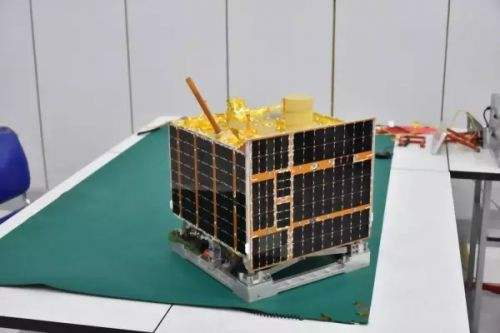
\includegraphics[width=9cm]{pic/tiantuo3.jpg}
\caption{天拓三号卫星主星吕梁一号\protect\footnotemark}
\label{fig:tiantuo3}
\end{figure}

\footnotetext{图片来源:\url{http://www.cannews.com.cn/2015/1114/139804_2.shtml}}

“吕梁一号”是我国第一颗以地方城市命名的微纳卫星,主要开展新型星载船舶自动识别系统(AIS)信号接收、星载航空目标信号广播式自动相关监视系统(ADS-B)信号接收、火灾监测、20 公斤级通用化卫星平台技术等系列科学试验和新技术验证。它是“吕梁号新型船舶自动识别信号接收系统”中的首颗微纳卫星。该系统能对全球范围船舶快速完成位置、航向、航速等信息的接收,实现了对我国现有岸基 AIS 系统的有效补充。航空目标信号接收的星载 ADS-B 则可对全球范围航空目标实行准实时目标监控、空中流量测量,为航线优化和提高航空飞行效率提供信息服务,这是我国首次开展此项卫星载荷在轨试验。

\subsection{实验结果}

据介绍,主星“吕梁一号”平均每天可接收全球范围 40 多万条 ADS-B 报文数据,幅宽超过 2000 公里,从每条报文中可以识别该航空目标的机型、代码、位置、速度、高度和航线等信息,数据清晰,航线及密度一目了然。

目前“吕梁一号”在轨运行状态良好,ADS-B 报文数据接收稳定,系统已实现业务运行,正在根据有关用户需求开展航空信号报文服务。有关专家指出,有了星载 ADS-B 系统,就能有效避免“马航”、“亚航”失联这样的事件,还能从其海量数据中分析提取对航空管制、物流监控、经济形势有潜在价值的信息。

“吕梁一号”微纳卫星成功发射,标志着山西吕梁市与国防科大落实军民融合战略取得标志性成果。

2013 年,国防科大吕梁军民融合协同创新研究院联合国防科大航天科学与工程学院组建山西省微纳卫星工程技术研究中心,开展星载船舶自动识别信号接收微纳卫星系统研制。“吕梁一号”的成功发射,不仅是吕梁发展史上卫星发射零的突破,也标志着吕梁市与国防科技大学在军民融合协同创新上迈出了重要一步,对推动我国军民融合发展具有积极的示范和促进作用。下一步,微纳卫星工程技术研究中心将研制发射多颗微纳卫星并实现多星组网,获取全球船舶动态数据,建立全球船舶动态数据库,同时推广微纳卫星的技术应用,带动相关产业的发展。\upcite{h10}

